% \vspace{0.1cm}  % 添加0.1厘米的垂直空间
% 
% \begin{table}[h]  % 开始表格环境,h表示尽量将表格放在当前位置
% 	\renewcommand{\arraystretch}{1.5}  % 设置表格行距为1.5倍
% 	\centering  % 表格居中
% 	\bicaption[\xiaosi 电流类型对效率的影响]{\wuhao 电流类型对效率的影响}{\wuhao Current type impact on efficiency}  % 双语标题,方括号内是目录中显示的标题(小四号字),第一个花括号内是中文标题(五号字),第二个花括号内是英文标题(五号字)
% 	\begin{tabular}{p{3cm}p{3cm}p{3cm}p{3cm}}  % 开始表格内容,定义4列,每列宽度为3厘米,p表示允许文本自动换行
% 		\toprule[1.5pt]  % 顶部粗线,粗细为1.5pt
% 		\makecell[c]{\songti\wuhao 电流类型}&\makecell[c]{\songti\wuhao A}&\makecell[c]{\songti\wuhao B}&\makecell[c]{\songti\wuhao C}\\  % 表头行,\makecell[c]表示单元格内容居中,\songti表示宋体,\wuhao表示五号字
% 		\hline  % 普通横线
% 		\makecell[c]{\wuhao aaa}&\makecell[c]{\wuhao aa1}&\makecell[c]{\wuhao bb1}&\makecell[c]{\wuhao cc1}\\  % 数据行,格式同上
% 		\bottomrule[1.5pt]  % 底部粗线,粗细为1.5pt
% 	\end{tabular}
%    \label{tab:3.1}  % 表格标签,用于交叉引用	
% \end{table}
%
% \vspace{-0.1cm}  % 调整表格与下文的间距




\begin{table}
	\centering
	\bicaption[\xiaosi 有无联邦学习的PU学习性能比较]{\wuhao 有无联邦学习的PU学习性能比较}{\wuhao Performance comparison of PU Learning with and without federation}
	\label{RQ1}
	\resizebox{\textwidth}{!}{
		{\songti \wuhao
			\begin{tabular}{llllllll} 
				\toprule[1.5pt]
				\multirow{2}{*}{Base Estimator} & \multirow{2}{*}{Metrics} & \multicolumn{2}{l}{The Bank Marketing} & \multicolumn{2}{l}{\begin{tabular}[c]{@{}l@{}}The Default of \\Credit Card Clients\end{tabular}} & \multicolumn{2}{l}{The Adult Census}  \\ 
				\cline{3-8}
				&                          & Fed   & No\_Fed                        & Fed   & No\_Fed                                                                                  & Fed   & No\_Fed                       \\ 
				\hline
				\multirow{4}{*}{LR}             & acc~↑                    & 0.923 & 0.948                          & 0.822 & 0.843                                                                                    & 0.814 & 0.852                         \\
				& recall↑                  & 0.194 & 0.219                          & 0.179 & 0.206                                                                                    & 0.126 & 0.141                         \\
				& precision↑               & 0.520 & 0.546                          & 0.502 & 0.513                                                                                    & 0.804 & 0.820                         \\
				& AUC↑                     & 0.658 & 0.685                          & 0.621 & 0.643                                                                                    & 0.854 & 0.858                         \\
				\multirow{4}{*}{RF}             & acc~↑                    & 0.935 & 0.952                          & 0.826 & 0.851                                                                                    & 0.848 & 0.852                         \\
				& recall↑                  & 0.219 & 0.248                          & 0.190 & 0.212                                                                                    & 0.154 & 0.165                         \\
				& precision↑               & 0.587 & 0.613                          & 0.546 & 0.562                                                                                    & 0.755 & 0.770                         \\
				& AUC↑                     & 0.882 & 0.909                          & 0.625 & 0.639                                                                                    & 0.805 & 0.854                         \\
				\multirow{4}{*}{GBDT}           & acc~↑                    & 0.943 & 0.945                          & 0.847 & 0.851                                                                                    & 0.862 & 0.873                         \\
				& recall↑                  & 0.239 & 0.241                          & 0.224 & 0.229                                                                                    & 0.188 & 0.205                         \\
				& precision↑               & 0.594 & 0.599                          & 0.581 & 0.586                                                                                    & 0.922 & 0.933                         \\
				& AUC↑                     & 0.886 & 0.891                          & 0.639 & 0.647                                                                                    & 0.854 & 0.869                         \\
				\multirow{4}{*}{LGB}            & acc~↑                    & 0.896 & 0.914                          & 0.815 & 0.843                                                                                    & 0.828 & 0.852                         \\
				& recall↑                  & 0.186 & 0.197                          & 0.167 & 0.182                                                                                    & 0.142 & 0.155                         \\
				& precision↑               & 0.518 & 0.542                          & 0.496 & 0.524                                                                                    & 0.354 & 0.373                         \\
				& AUC↑                     & 0.587 & 0.612                          & 0.569 & 0.582                                                                                    & 0.705 & 0.721                         \\
				\toprule[1.5pt]
			\end{tabular}
		}
	}
\end{table}










% \begin{table}[h]  % 开始表格环境,h表示尽量将表格放在当前位置
% 	\renewcommand{\arraystretch}{1.5}  % 设置表格行距为1.5倍
% 	\centering  % 表格居中
% 	\bicaption[\xiaosi 电流类型对效率的影响]{\wuhao 电流类型对效率的影响}{\wuhao Current type impact on efficiency}  % 双语标题,方括号内是目录中显示的标题(小四号字),第一个花括号内是中文标题(五号字),第二个花括号内是英文标题(五号字)
% 	\begin{tabular}{p{3cm}p{3cm}p{3cm}p{3cm}}  % 开始表格内容,定义4列,每列宽度为3厘米,p表示允许文本自动换行
% 		\toprule[1.5pt]  % 顶部粗线,粗细为1.5pt
% 		\makecell[c]{\songti\wuhao 电流类型}&\makecell[c]{\songti\wuhao A}&\makecell[c]{\songti\wuhao B}&\makecell[c]{\songti\wuhao C}\\  % 表头行,\makecell[c]表示单元格内容居中,\songti表示宋体,\wuhao表示五号字
% 		\hline  % 普通横线
% 		\makecell[c]{\wuhao aaa}&\makecell[c]{\wuhao aa1}&\makecell[c]{\wuhao bb1}&\makecell[c]{\wuhao cc1}\\  % 数据行,格式同上
% 		\bottomrule[1.5pt]  % 底部粗线,粗细为1.5pt
% 	\end{tabular}
%    \label{tab:3.1}  % 表格标签,用于交叉引用	
% \end{table}




\begin{figure}[!htbp]
	\centering
%	\setlength{\subfigcapskip}{0.1cm}
	
	\captionsetup{size=footnotesize}
	\begin{subfigure}{0.45\textwidth}
		\centering
		\captionsetup{skip=1pt}
		\captionsetup{size=scriptsize}
		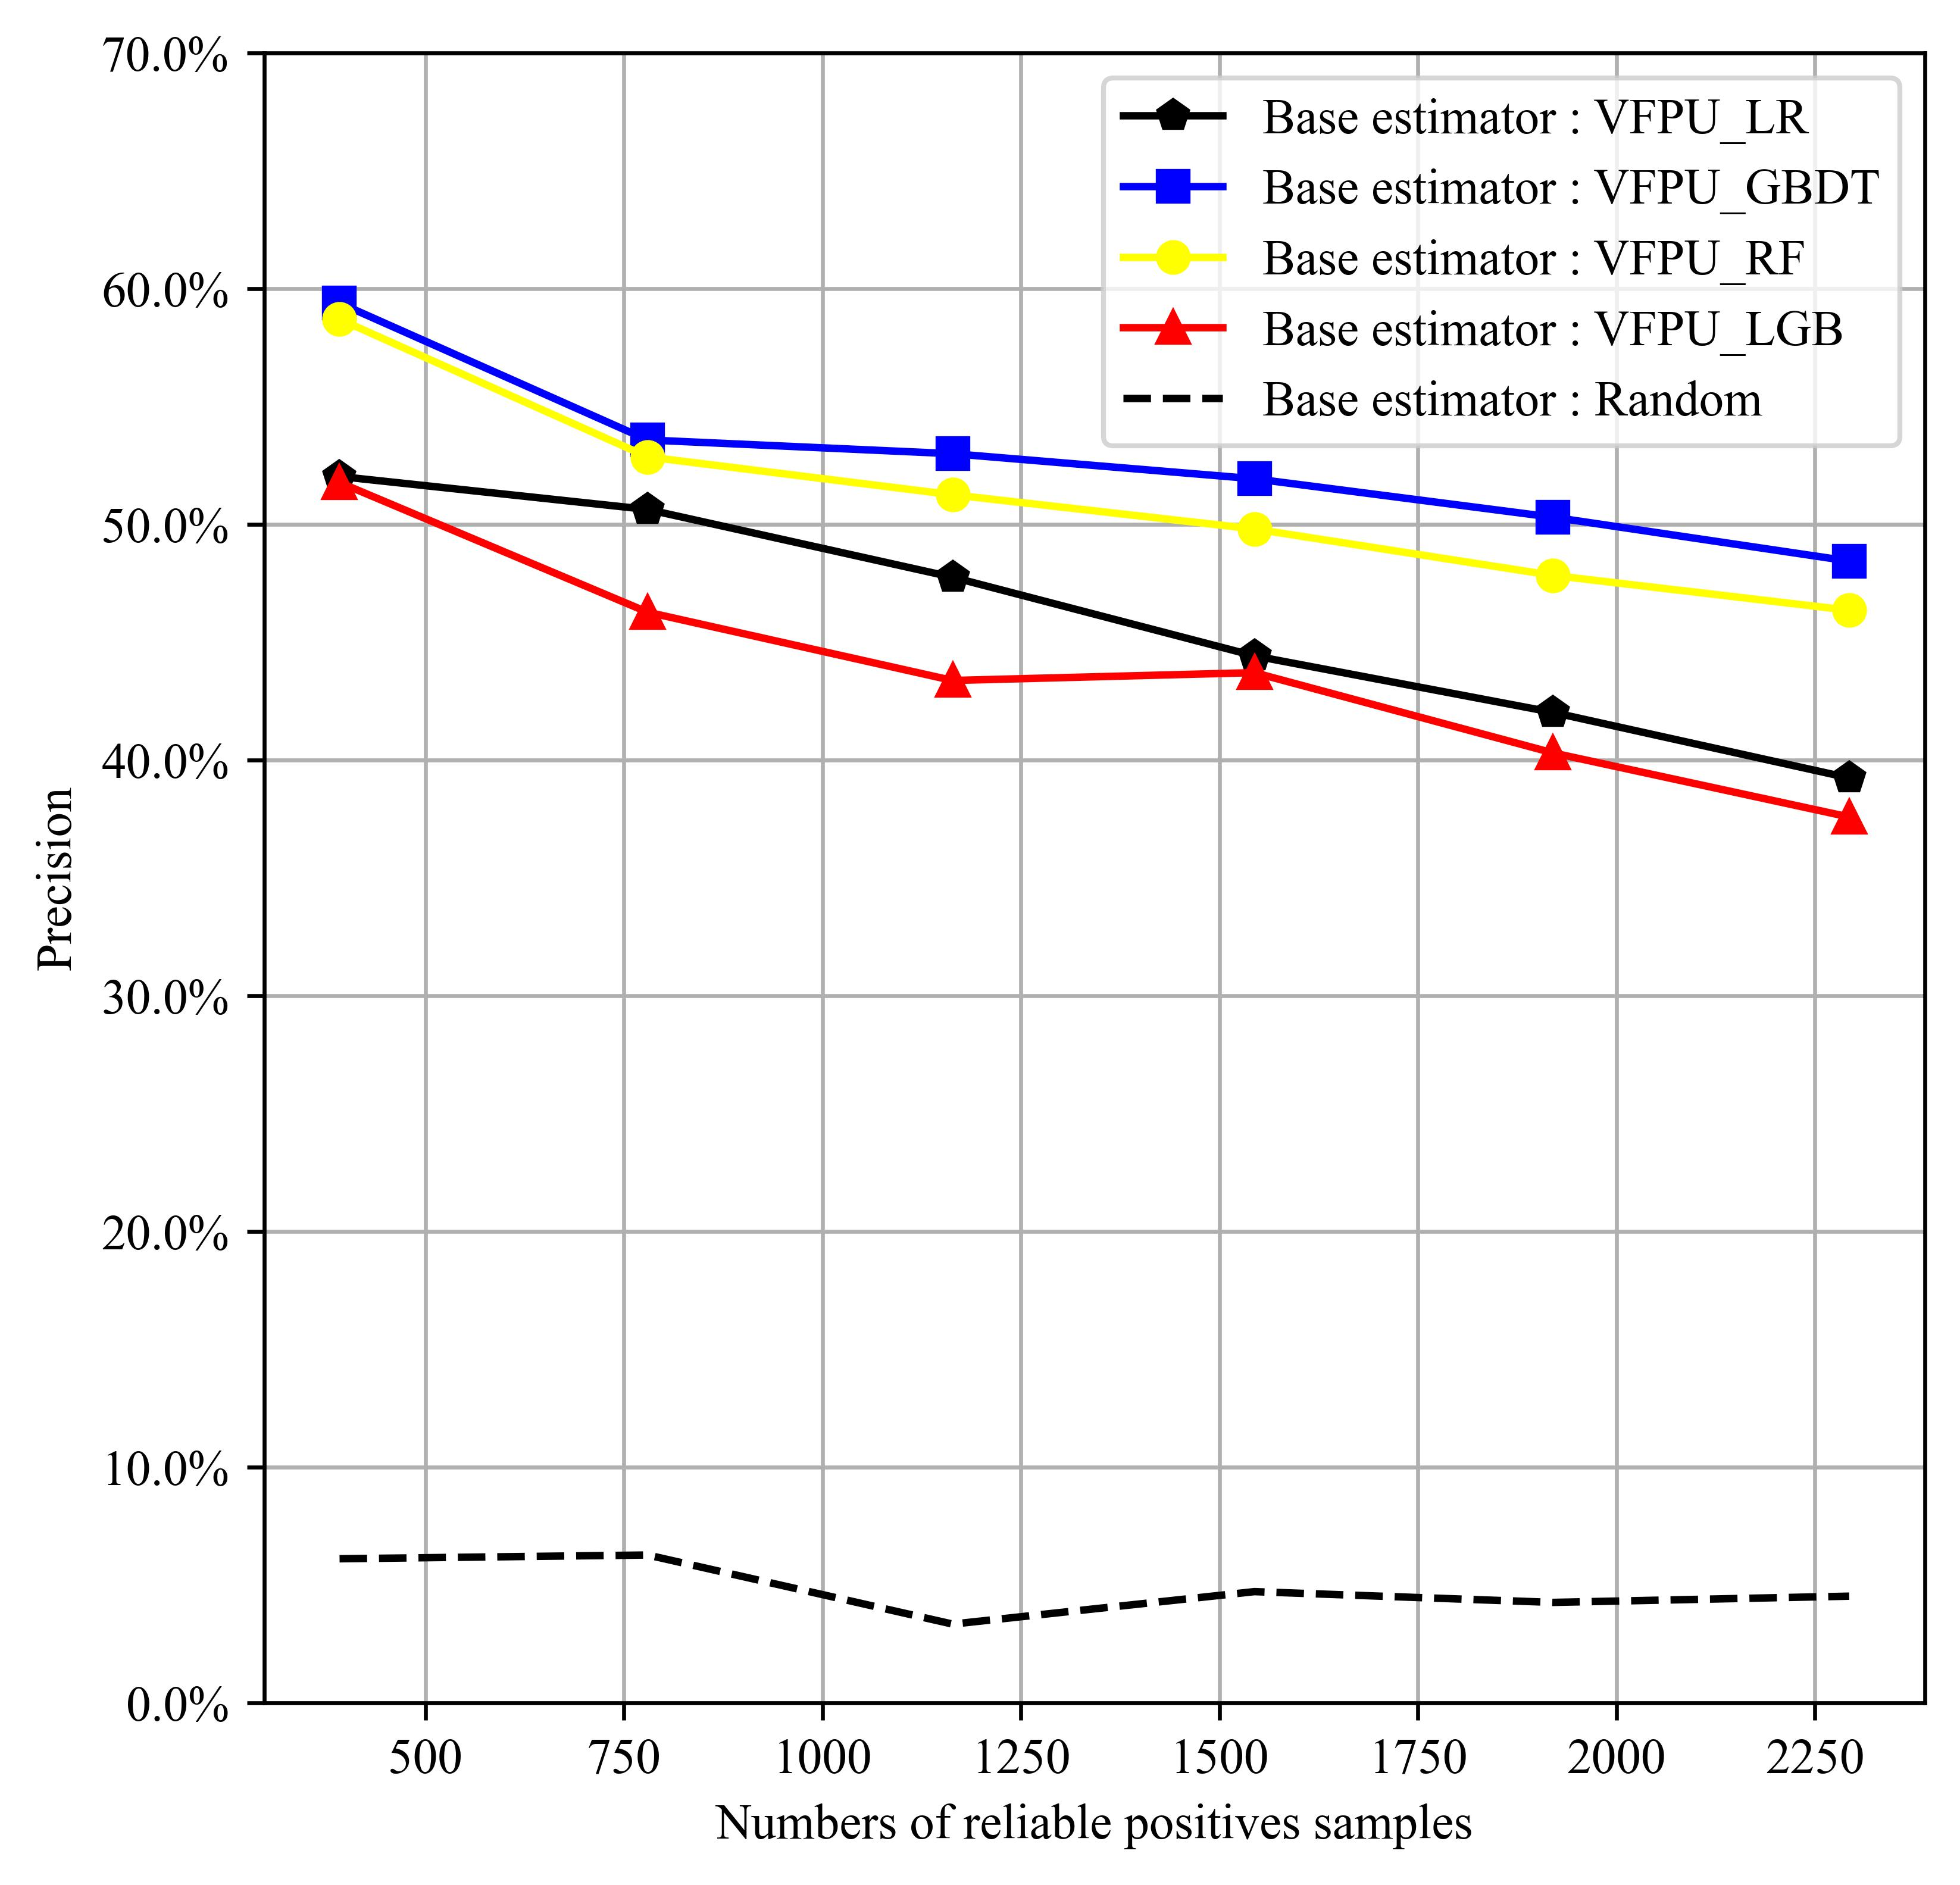
\includegraphics[width=0.9\textwidth,height=5.1cm]{chapters/imgs/Figure 2 (1) in JEPG format}
		\caption{Precision}
%		\vspace{0cm}
		\label{RQ2.1.sub1}
	\end{subfigure}
%	\hfill
%    \hspace{-1cm}
	\begin{subfigure}{0.45\textwidth}
		\centering
		\captionsetup{skip=4pt}
		\captionsetup{size=scriptsize}
		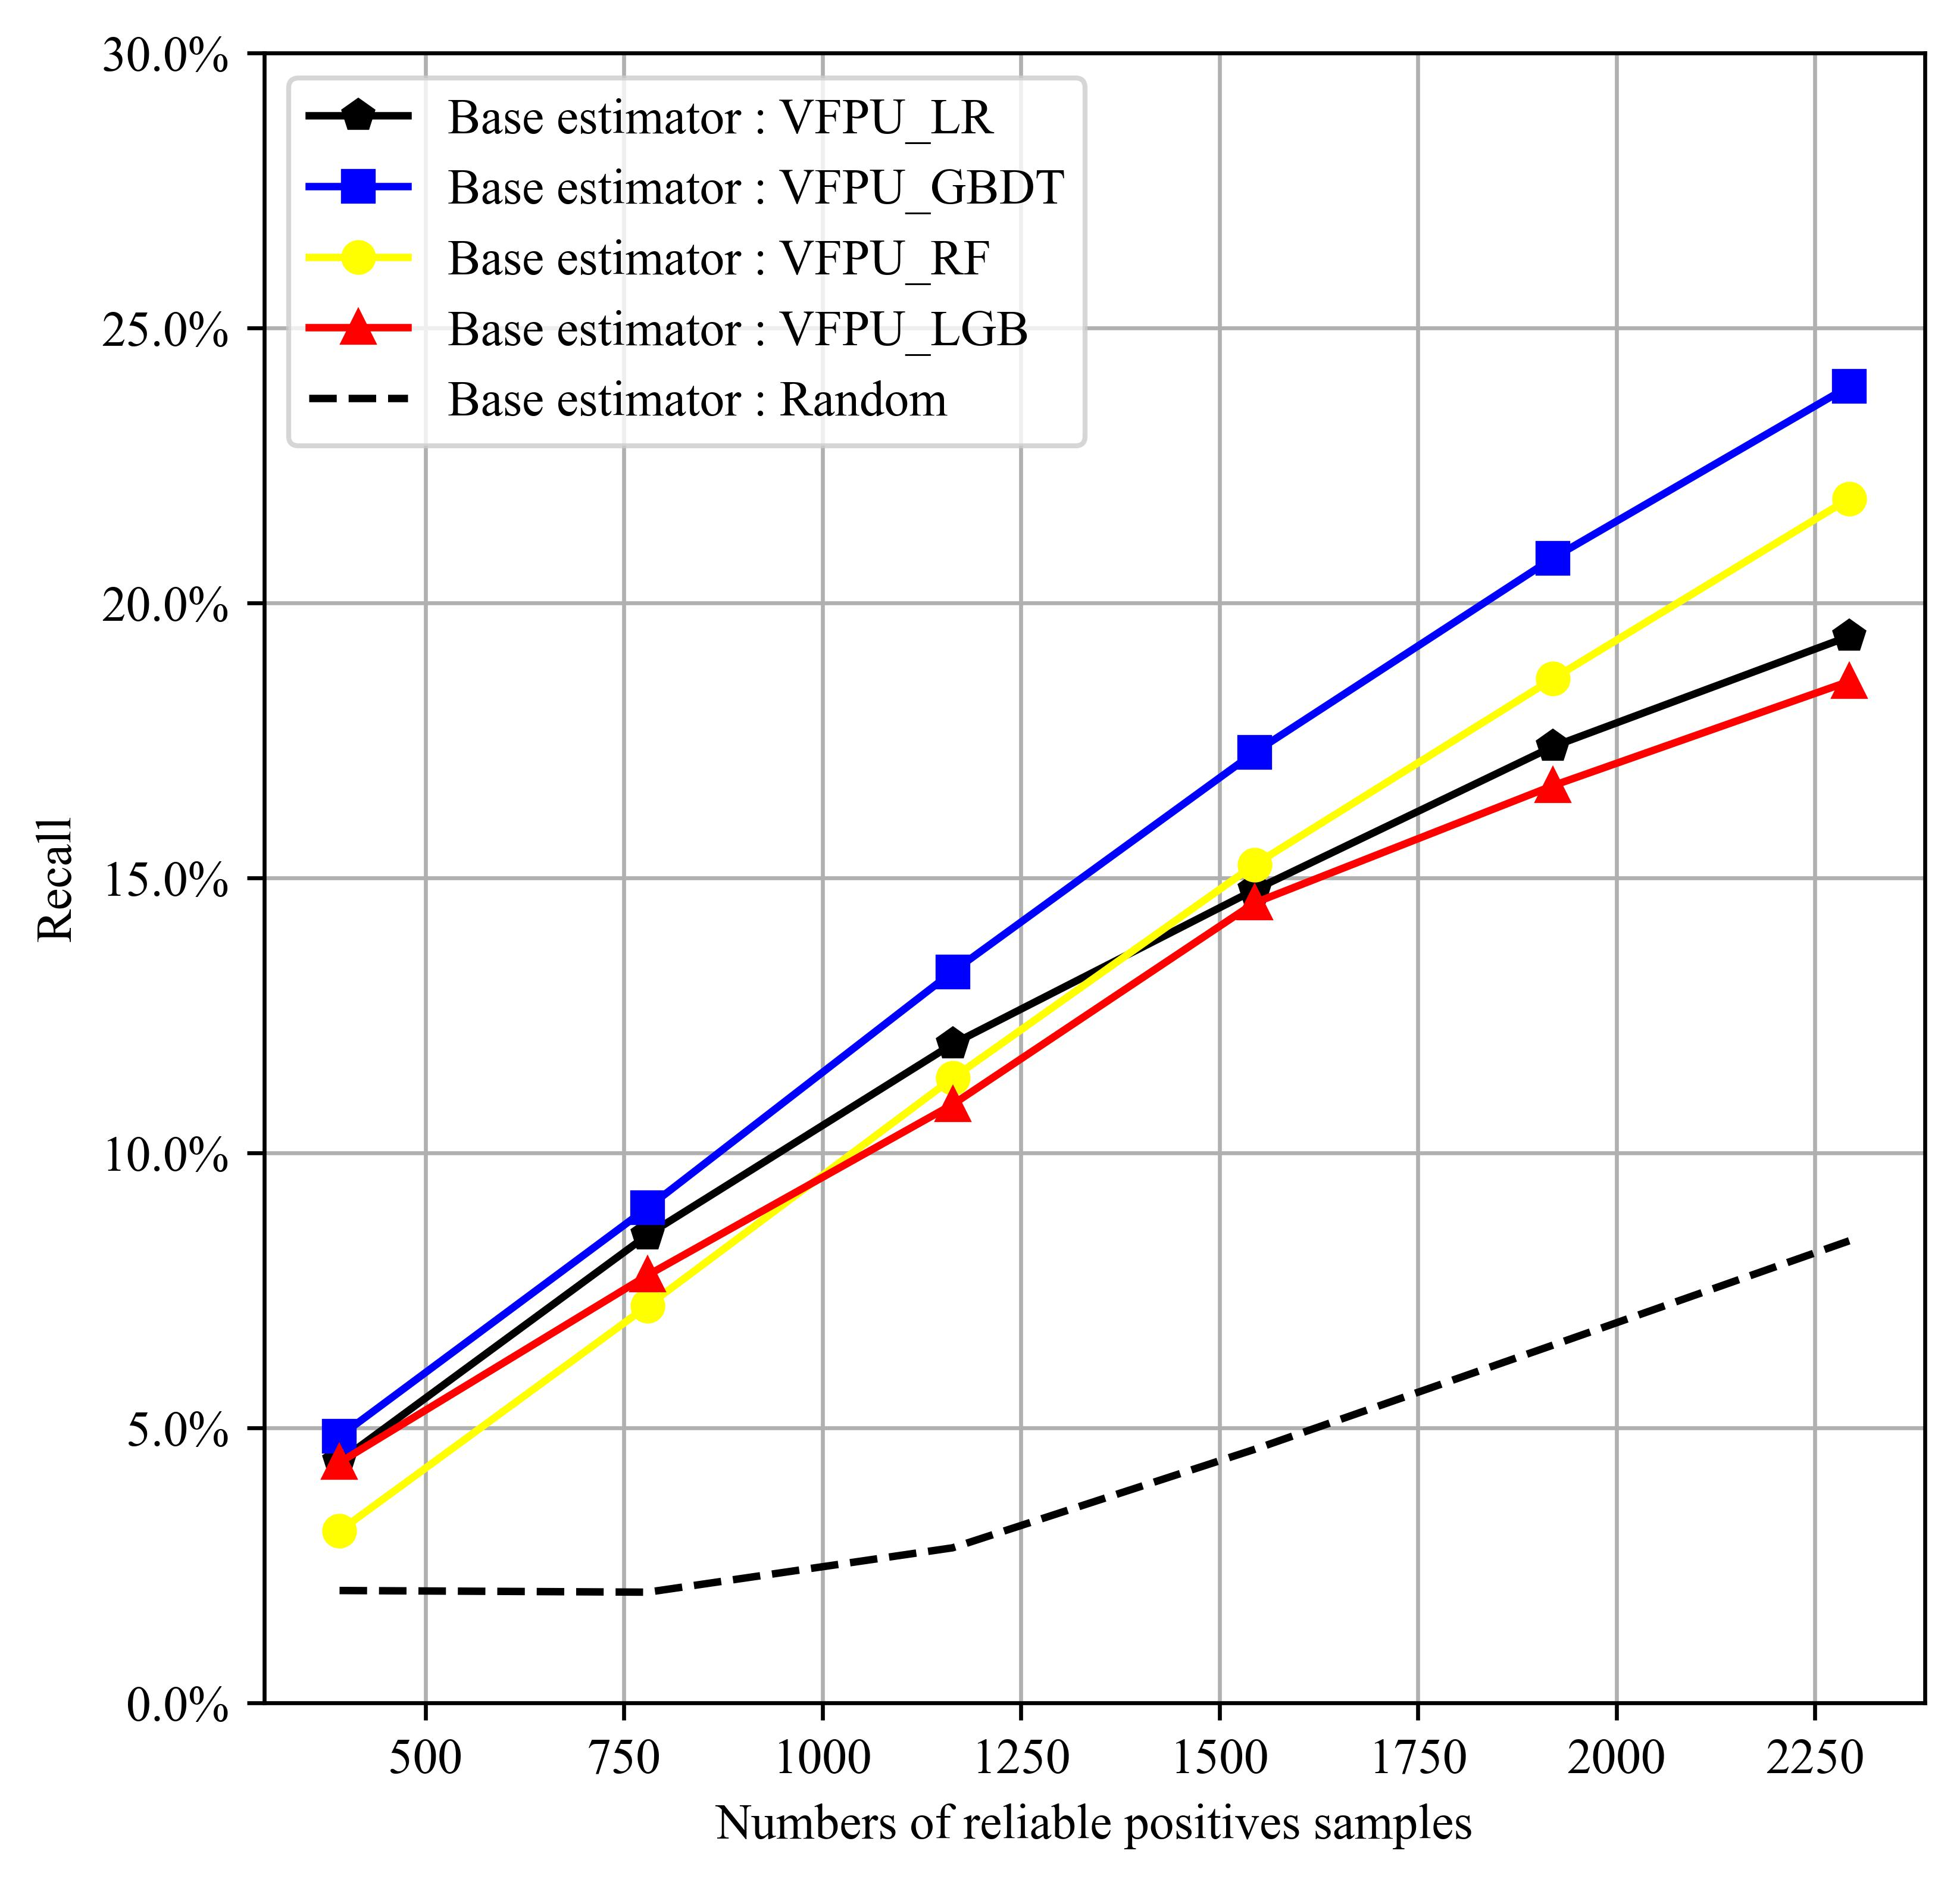
\includegraphics[width=0.9\textwidth,height=5.1cm]{chapters/imgs/Figure 2 (2) in JEPG format}
		\caption{Recall}
		\label{RQ2.1.sub2}
	\end{subfigure}
	
%	\vspace{0.05cm}
	
	\begin{subfigure}{0.45\textwidth}
		\centering
		\captionsetup{skip=4pt}
		\captionsetup{size=scriptsize}
		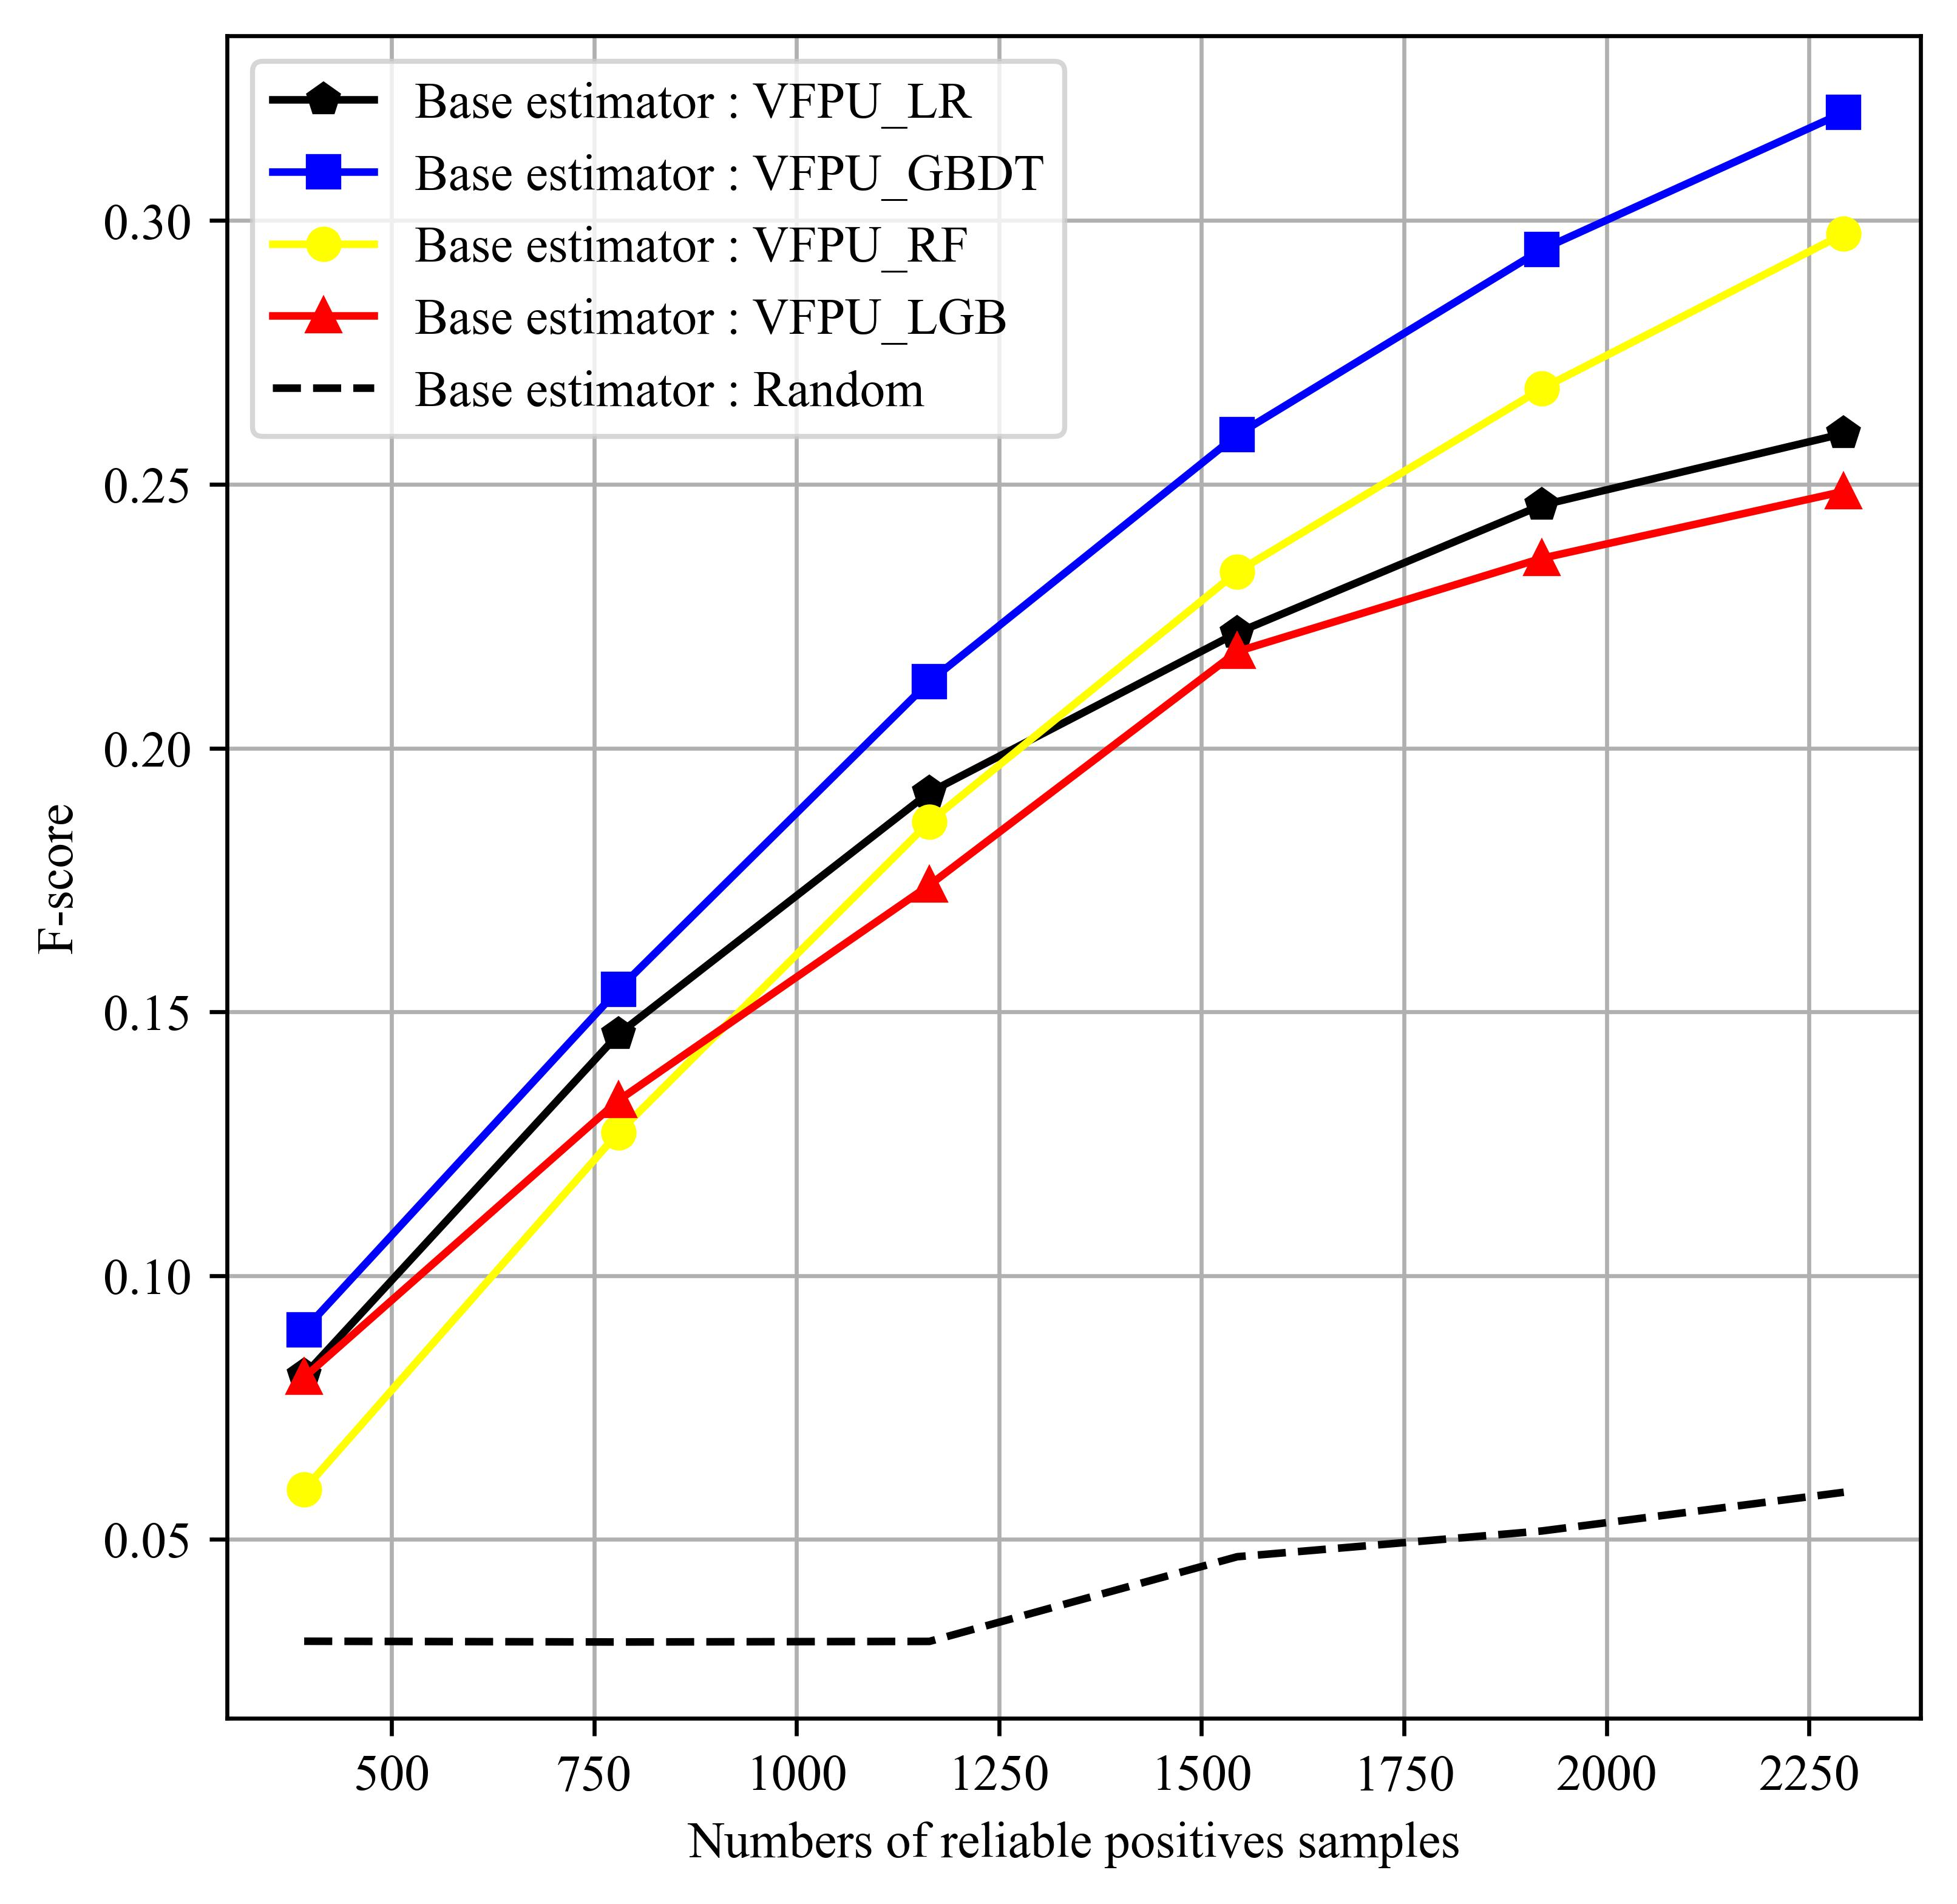
\includegraphics[width=0.9\textwidth,height=5.1cm]{chapters/imgs/Figure 2 (3) in JEPG format}
		\caption{F-score}
		\label{RQ2.1.sub3}
	\end{subfigure}
%\hfill
	\begin{subfigure}{0.45\textwidth}
		\centering
		\captionsetup{skip=4pt}
		\captionsetup{size=scriptsize}
		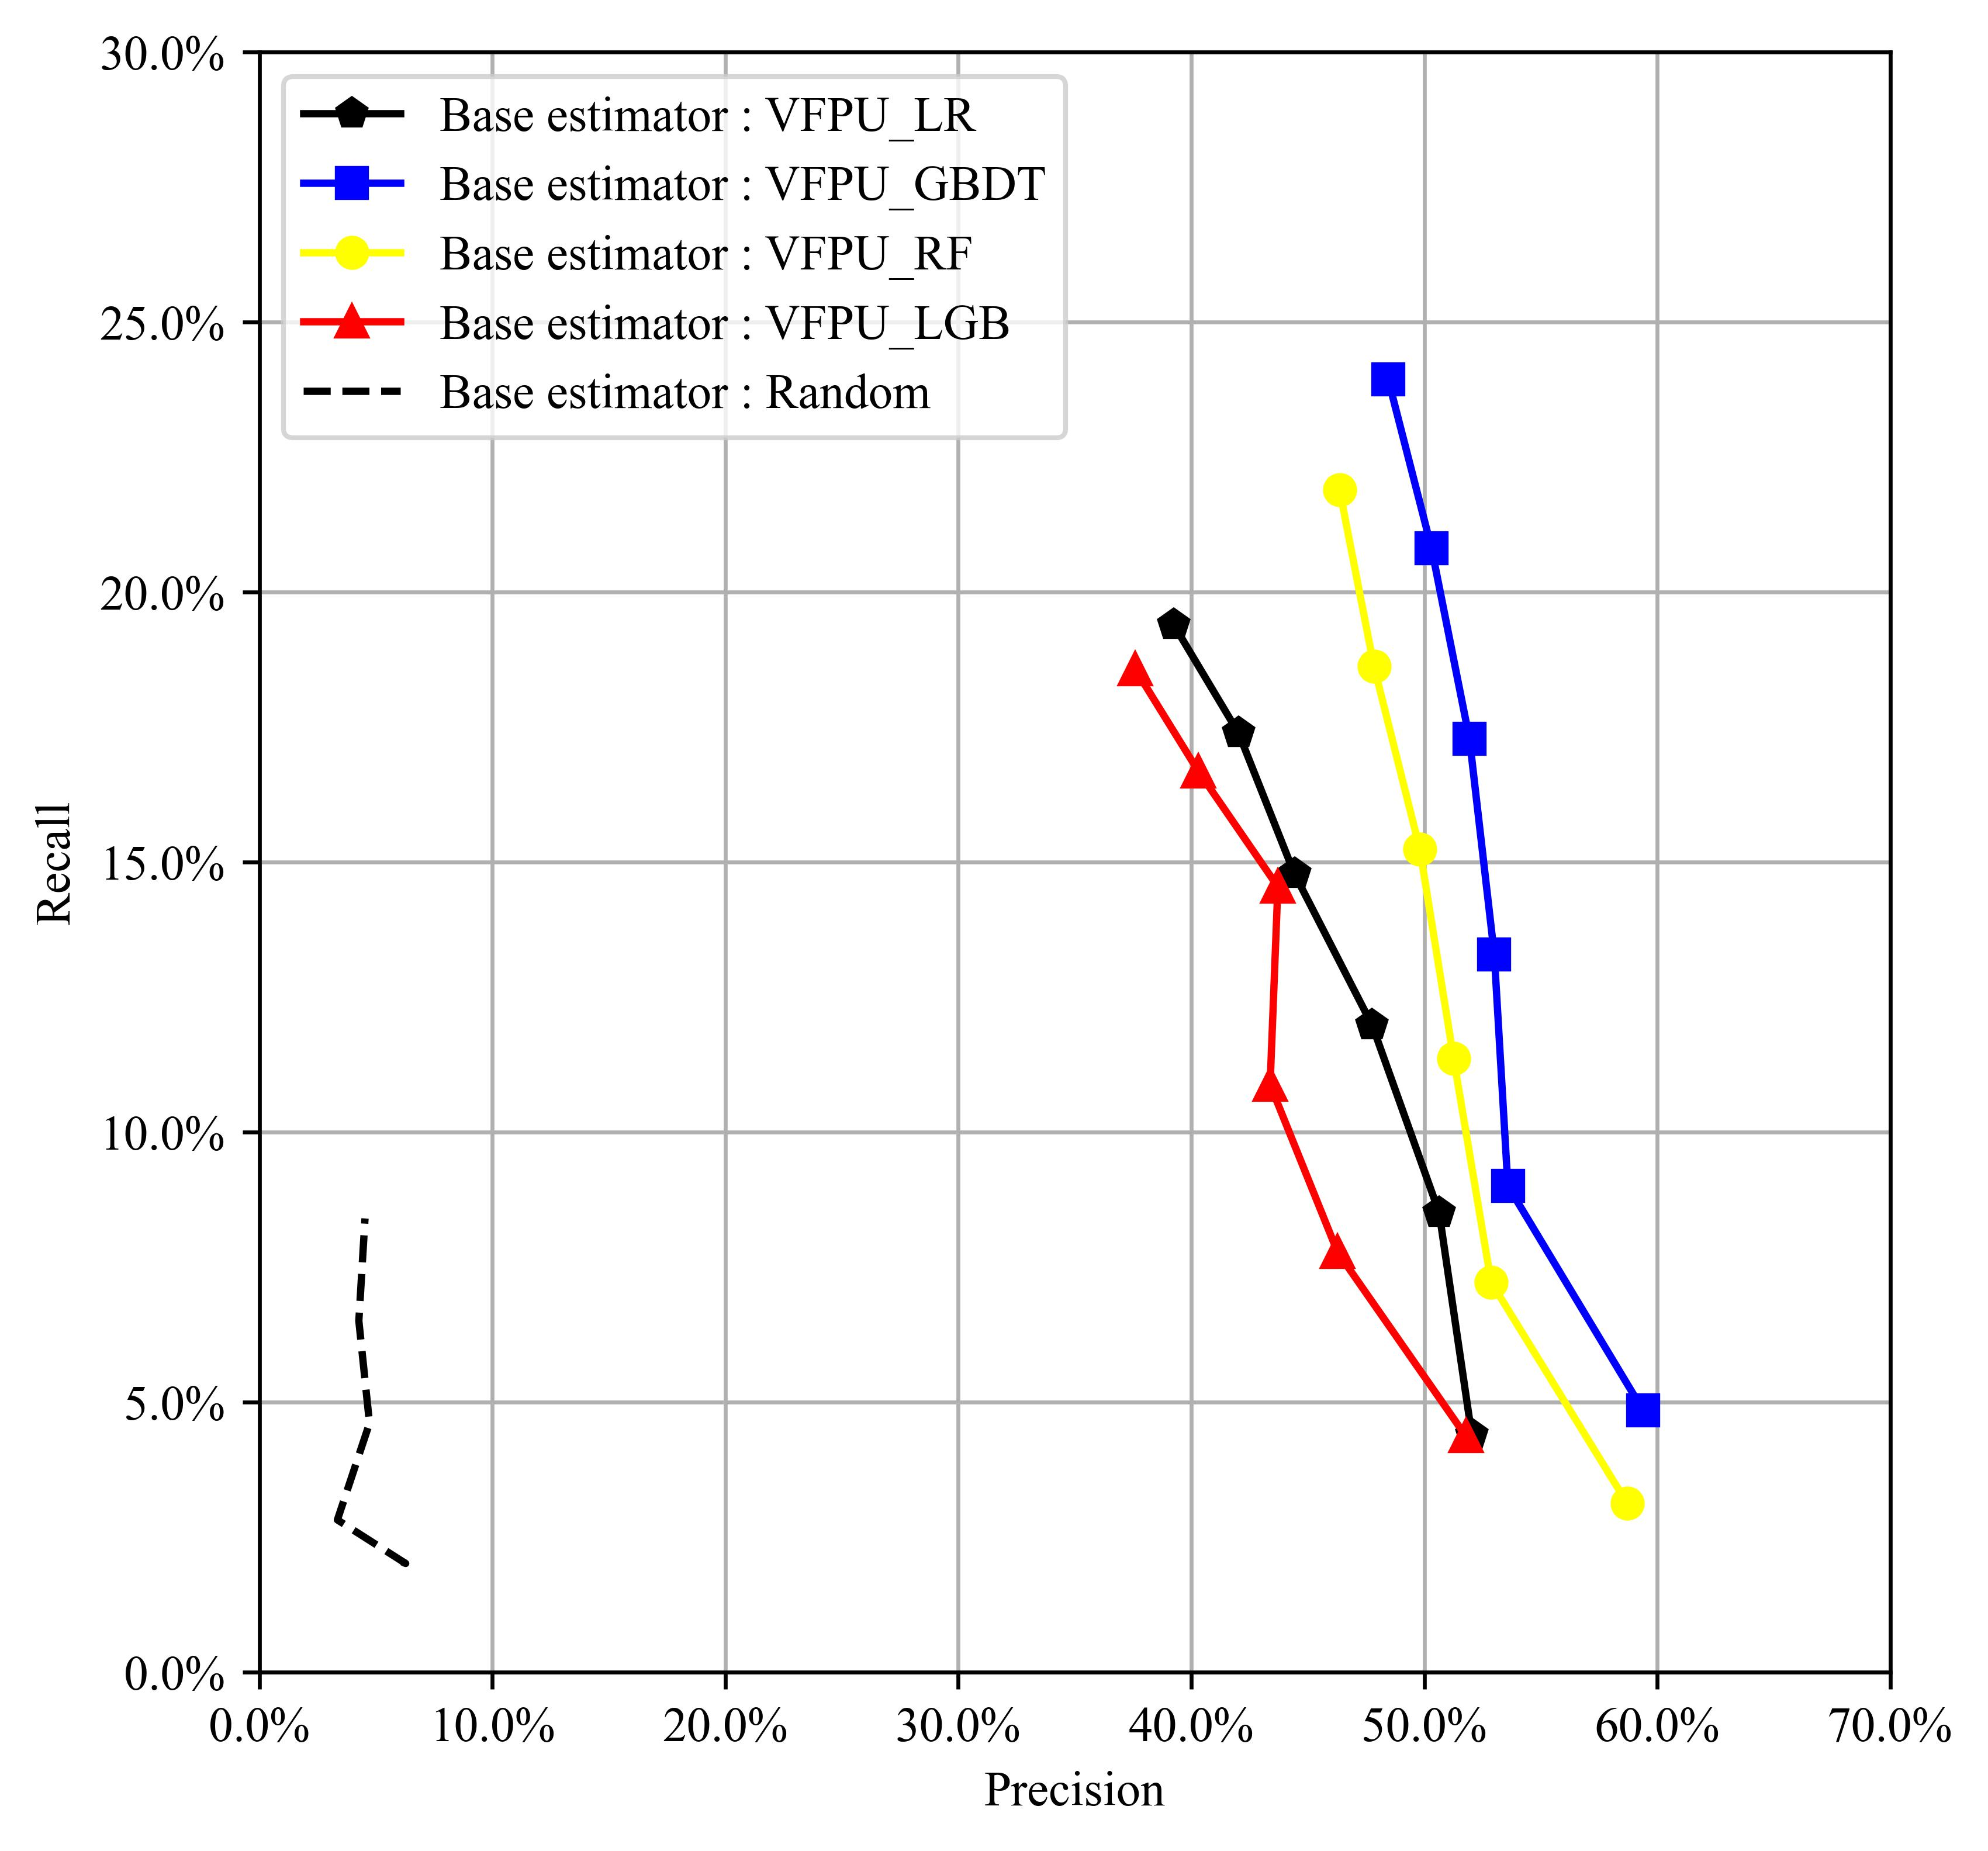
\includegraphics[width=0.95\textwidth,height=5.1cm]{chapters/imgs/Figure 2 (4) in JEPG format}
		\caption{Precision-Recall}
		\label{RQ2.1.sub4}
	\end{subfigure}
	
	\bicaption[\xiaosi 不同基学器在不同可靠正样本数量下的性能]{\wuhao 不同基学器在不同可靠正样本数量下的性能:(1)精度;(2)召回率;(3)F-score;(4)精度-召回率(Bank 数据集)}{\wuhao Performance of Different Base Estimators with Varying Reliable Positive Samples: (1) Precision; (2) Recall; (3) F-score; (4) Precision-Recall (The Bank Marketing Dataset)}
    \label{RQ2.1}
\end{figure}


\begin{figure}[!htbp]
	\centering
	\captionsetup{size=footnotesize}
	\begin{subfigure}{0.45\textwidth}
		\centering
		\captionsetup{skip=4pt}
		\captionsetup{size=scriptsize}
		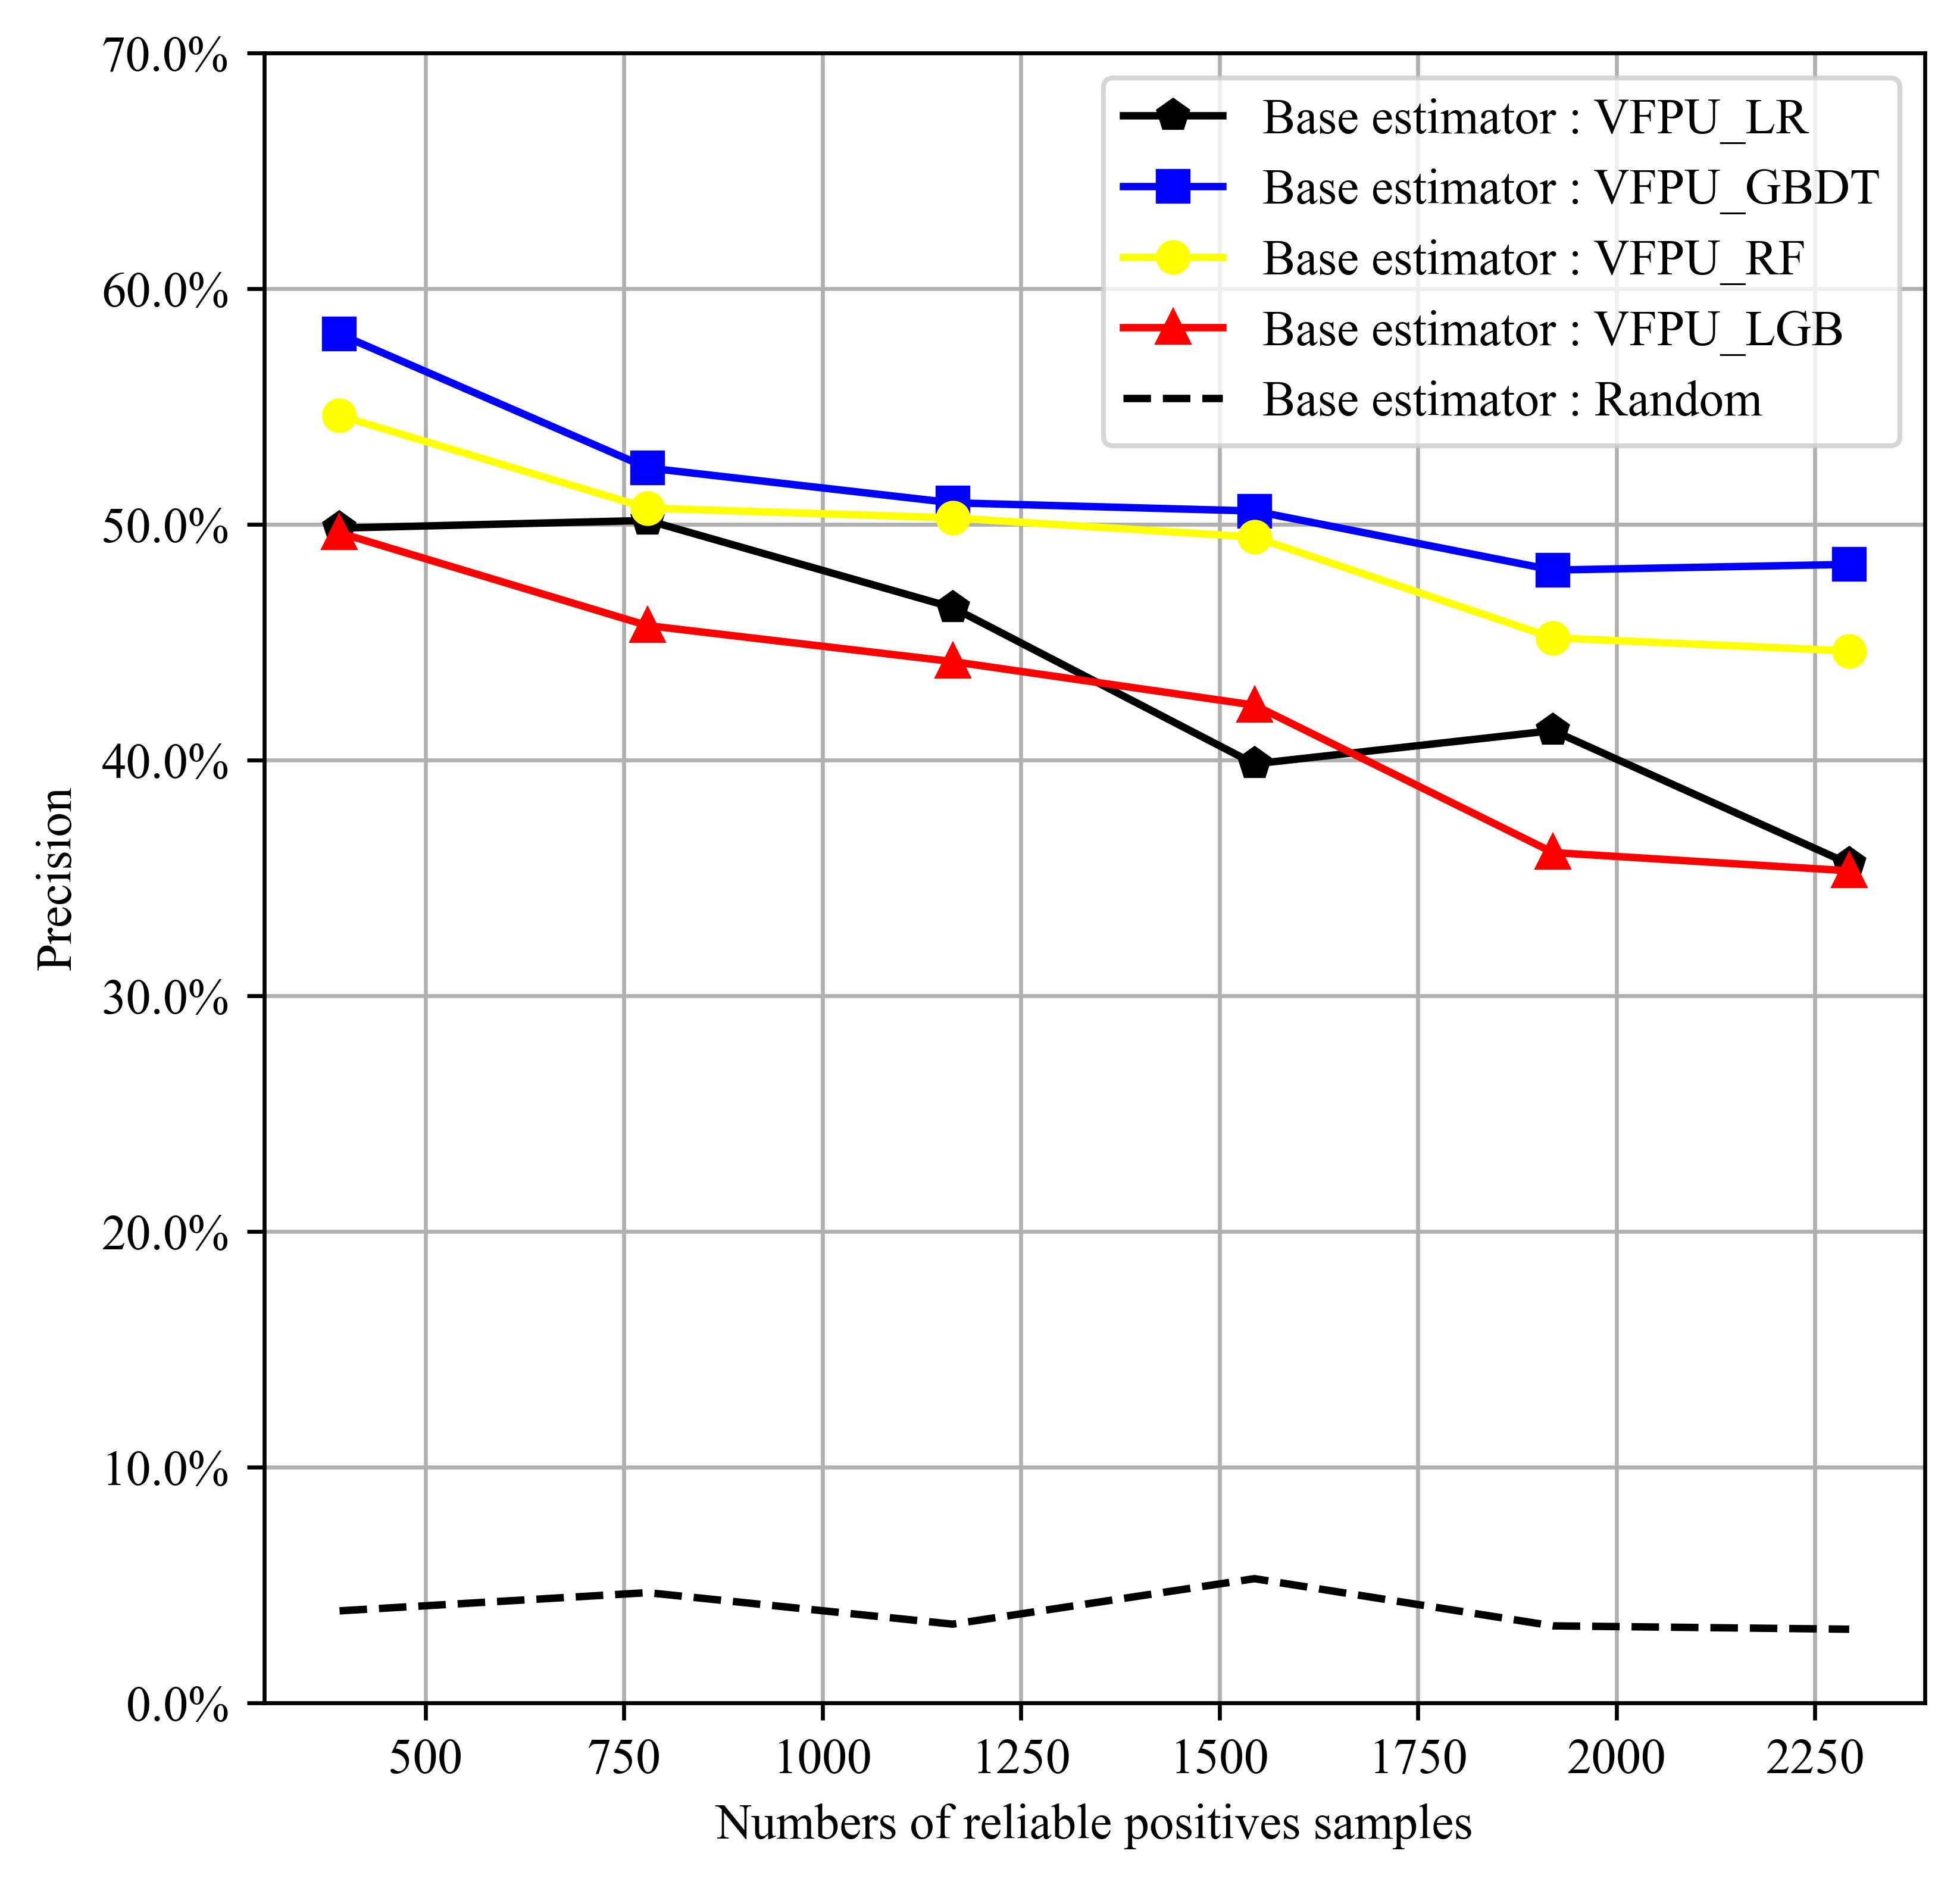
\includegraphics[width=0.9\textwidth,height=5.1cm]{chapters/imgs/Figure 3 (1) in JEPG format}
		\caption{Precision}
		\label{RQ2.2.sub1}
	\end{subfigure}
%\hfill
	\begin{subfigure}{0.45\textwidth}
		\centering
		\captionsetup{skip=4pt}
		\captionsetup{size=scriptsize}
		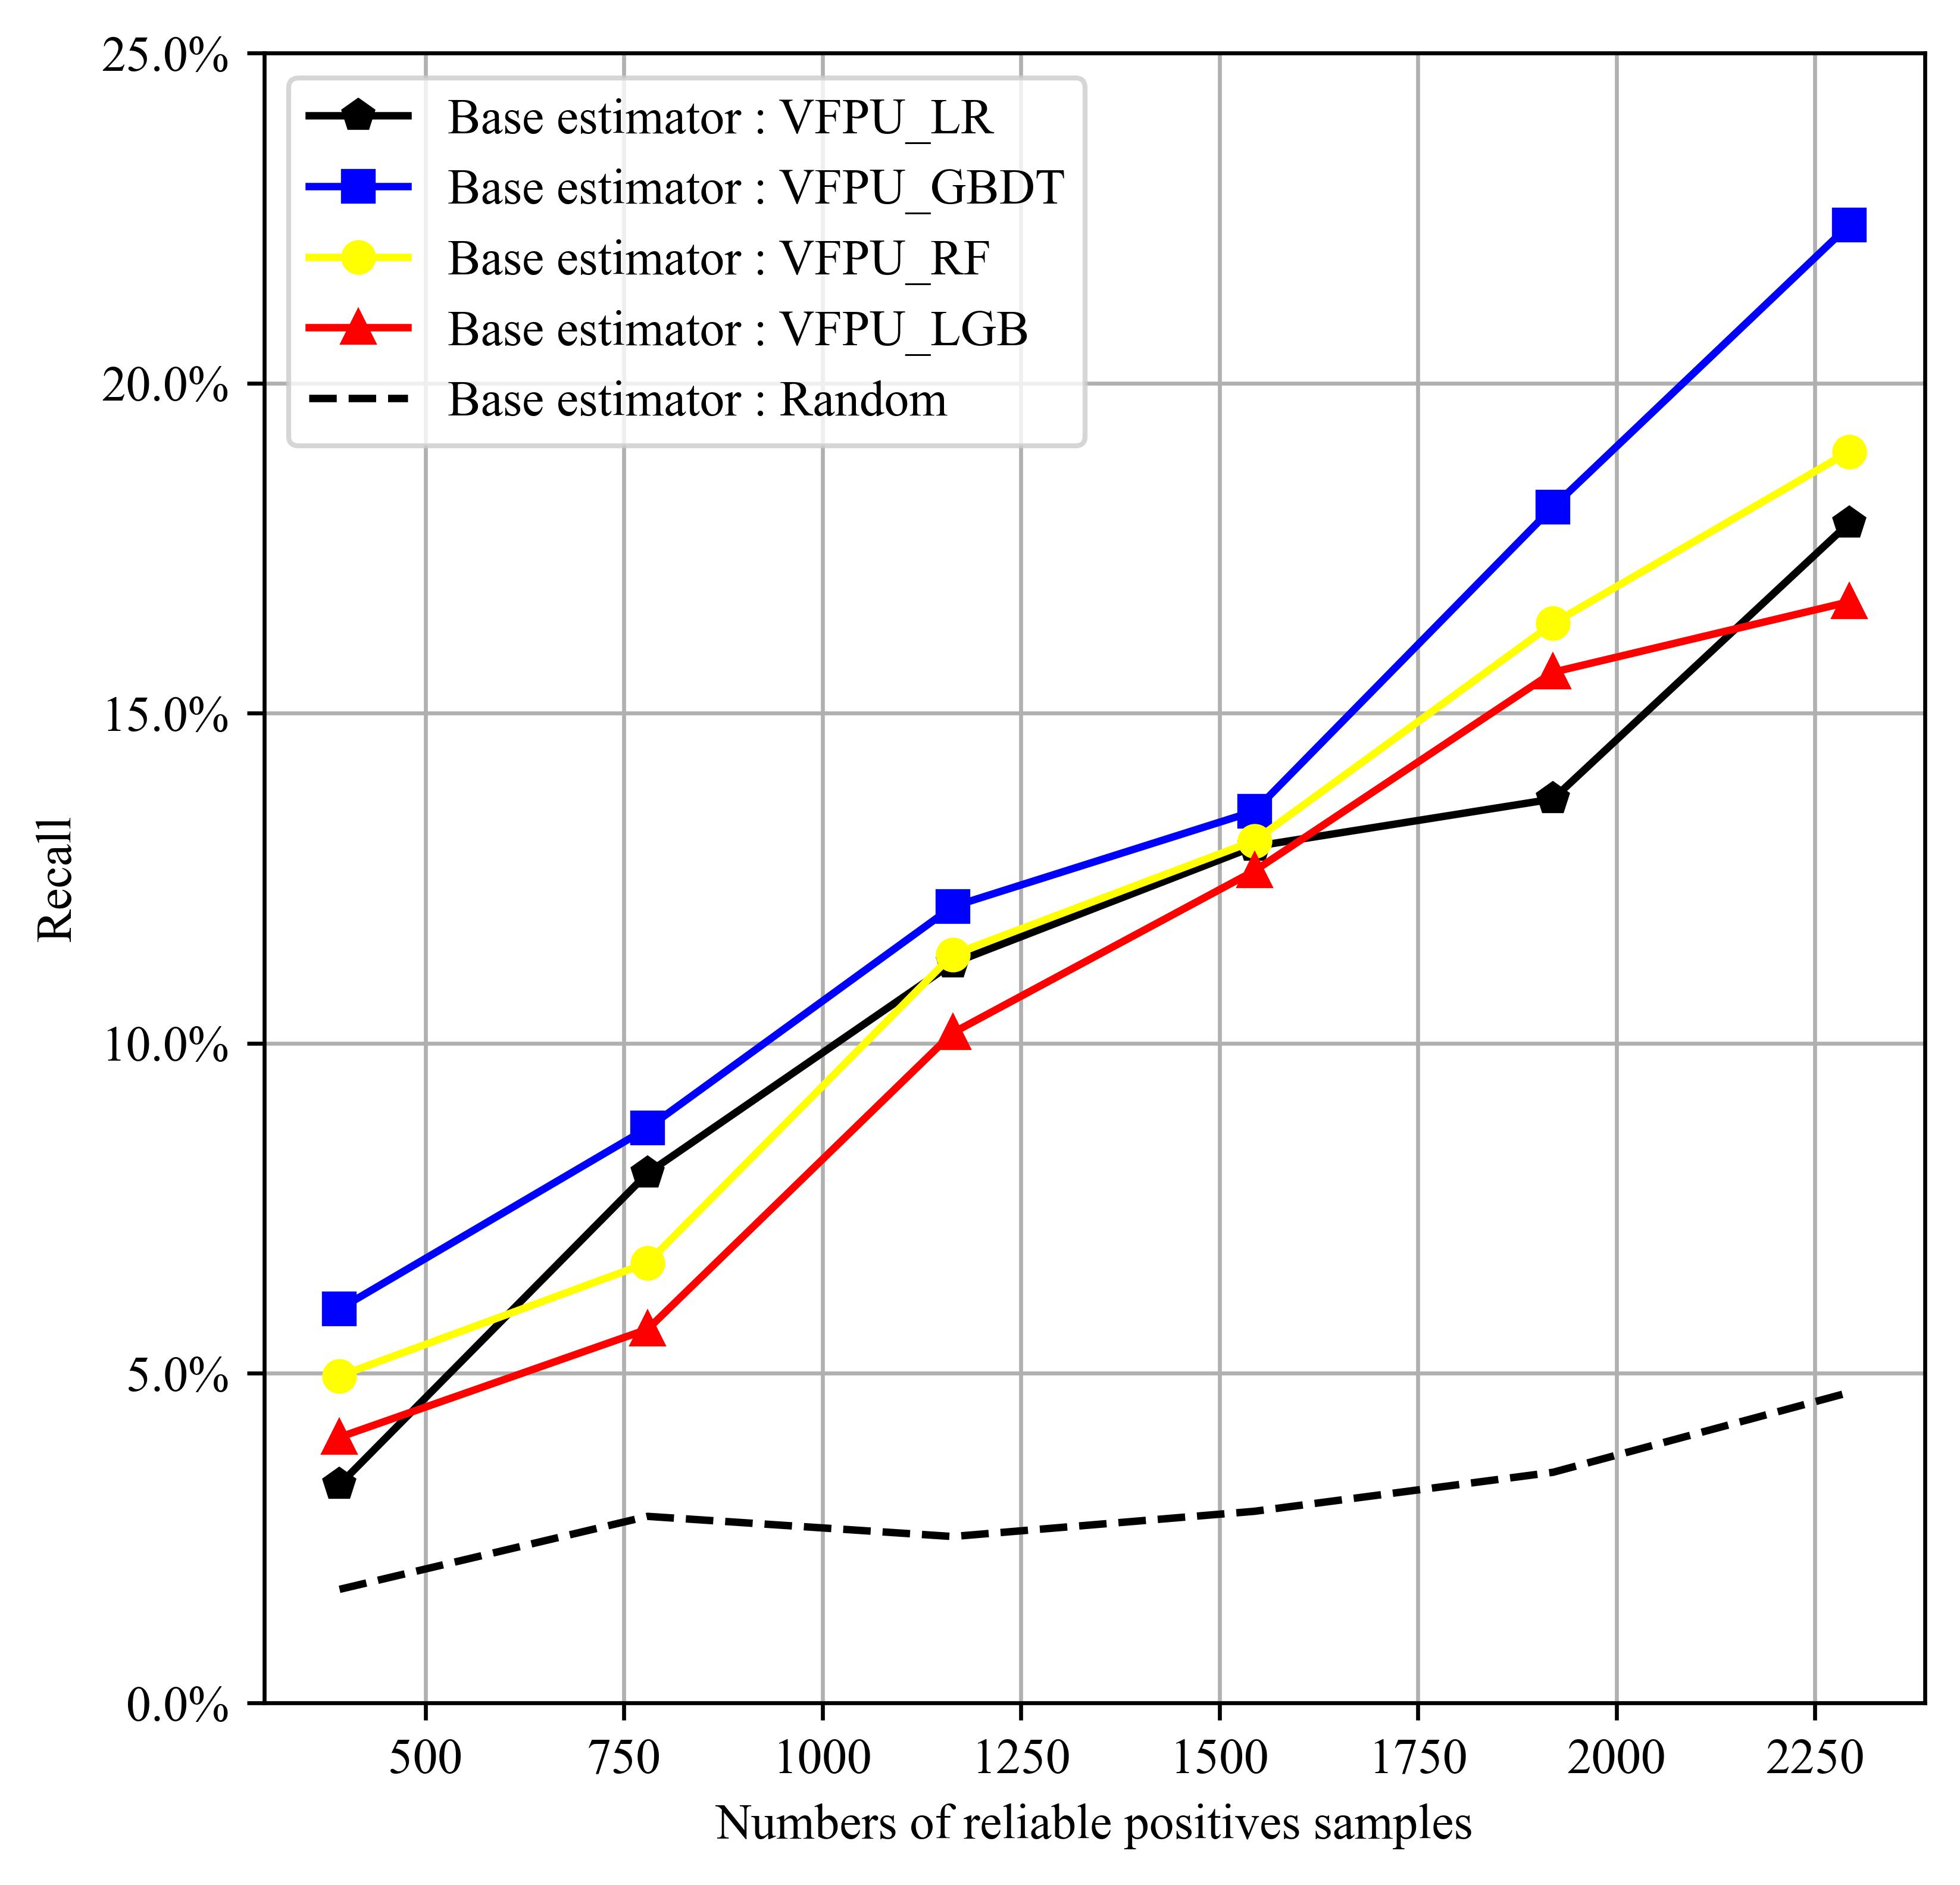
\includegraphics[width=0.9\textwidth,height=5.1cm]{chapters/imgs/Figure 3 (2) in JEPG format}
		\caption{Recall}
		\label{RQ2.2.sub2}
	\end{subfigure}
	
%	\vspace{0.05cm}
	
	\begin{subfigure}{0.45\textwidth}
		\centering
		\captionsetup{skip=4pt}
		\captionsetup{size=scriptsize}
		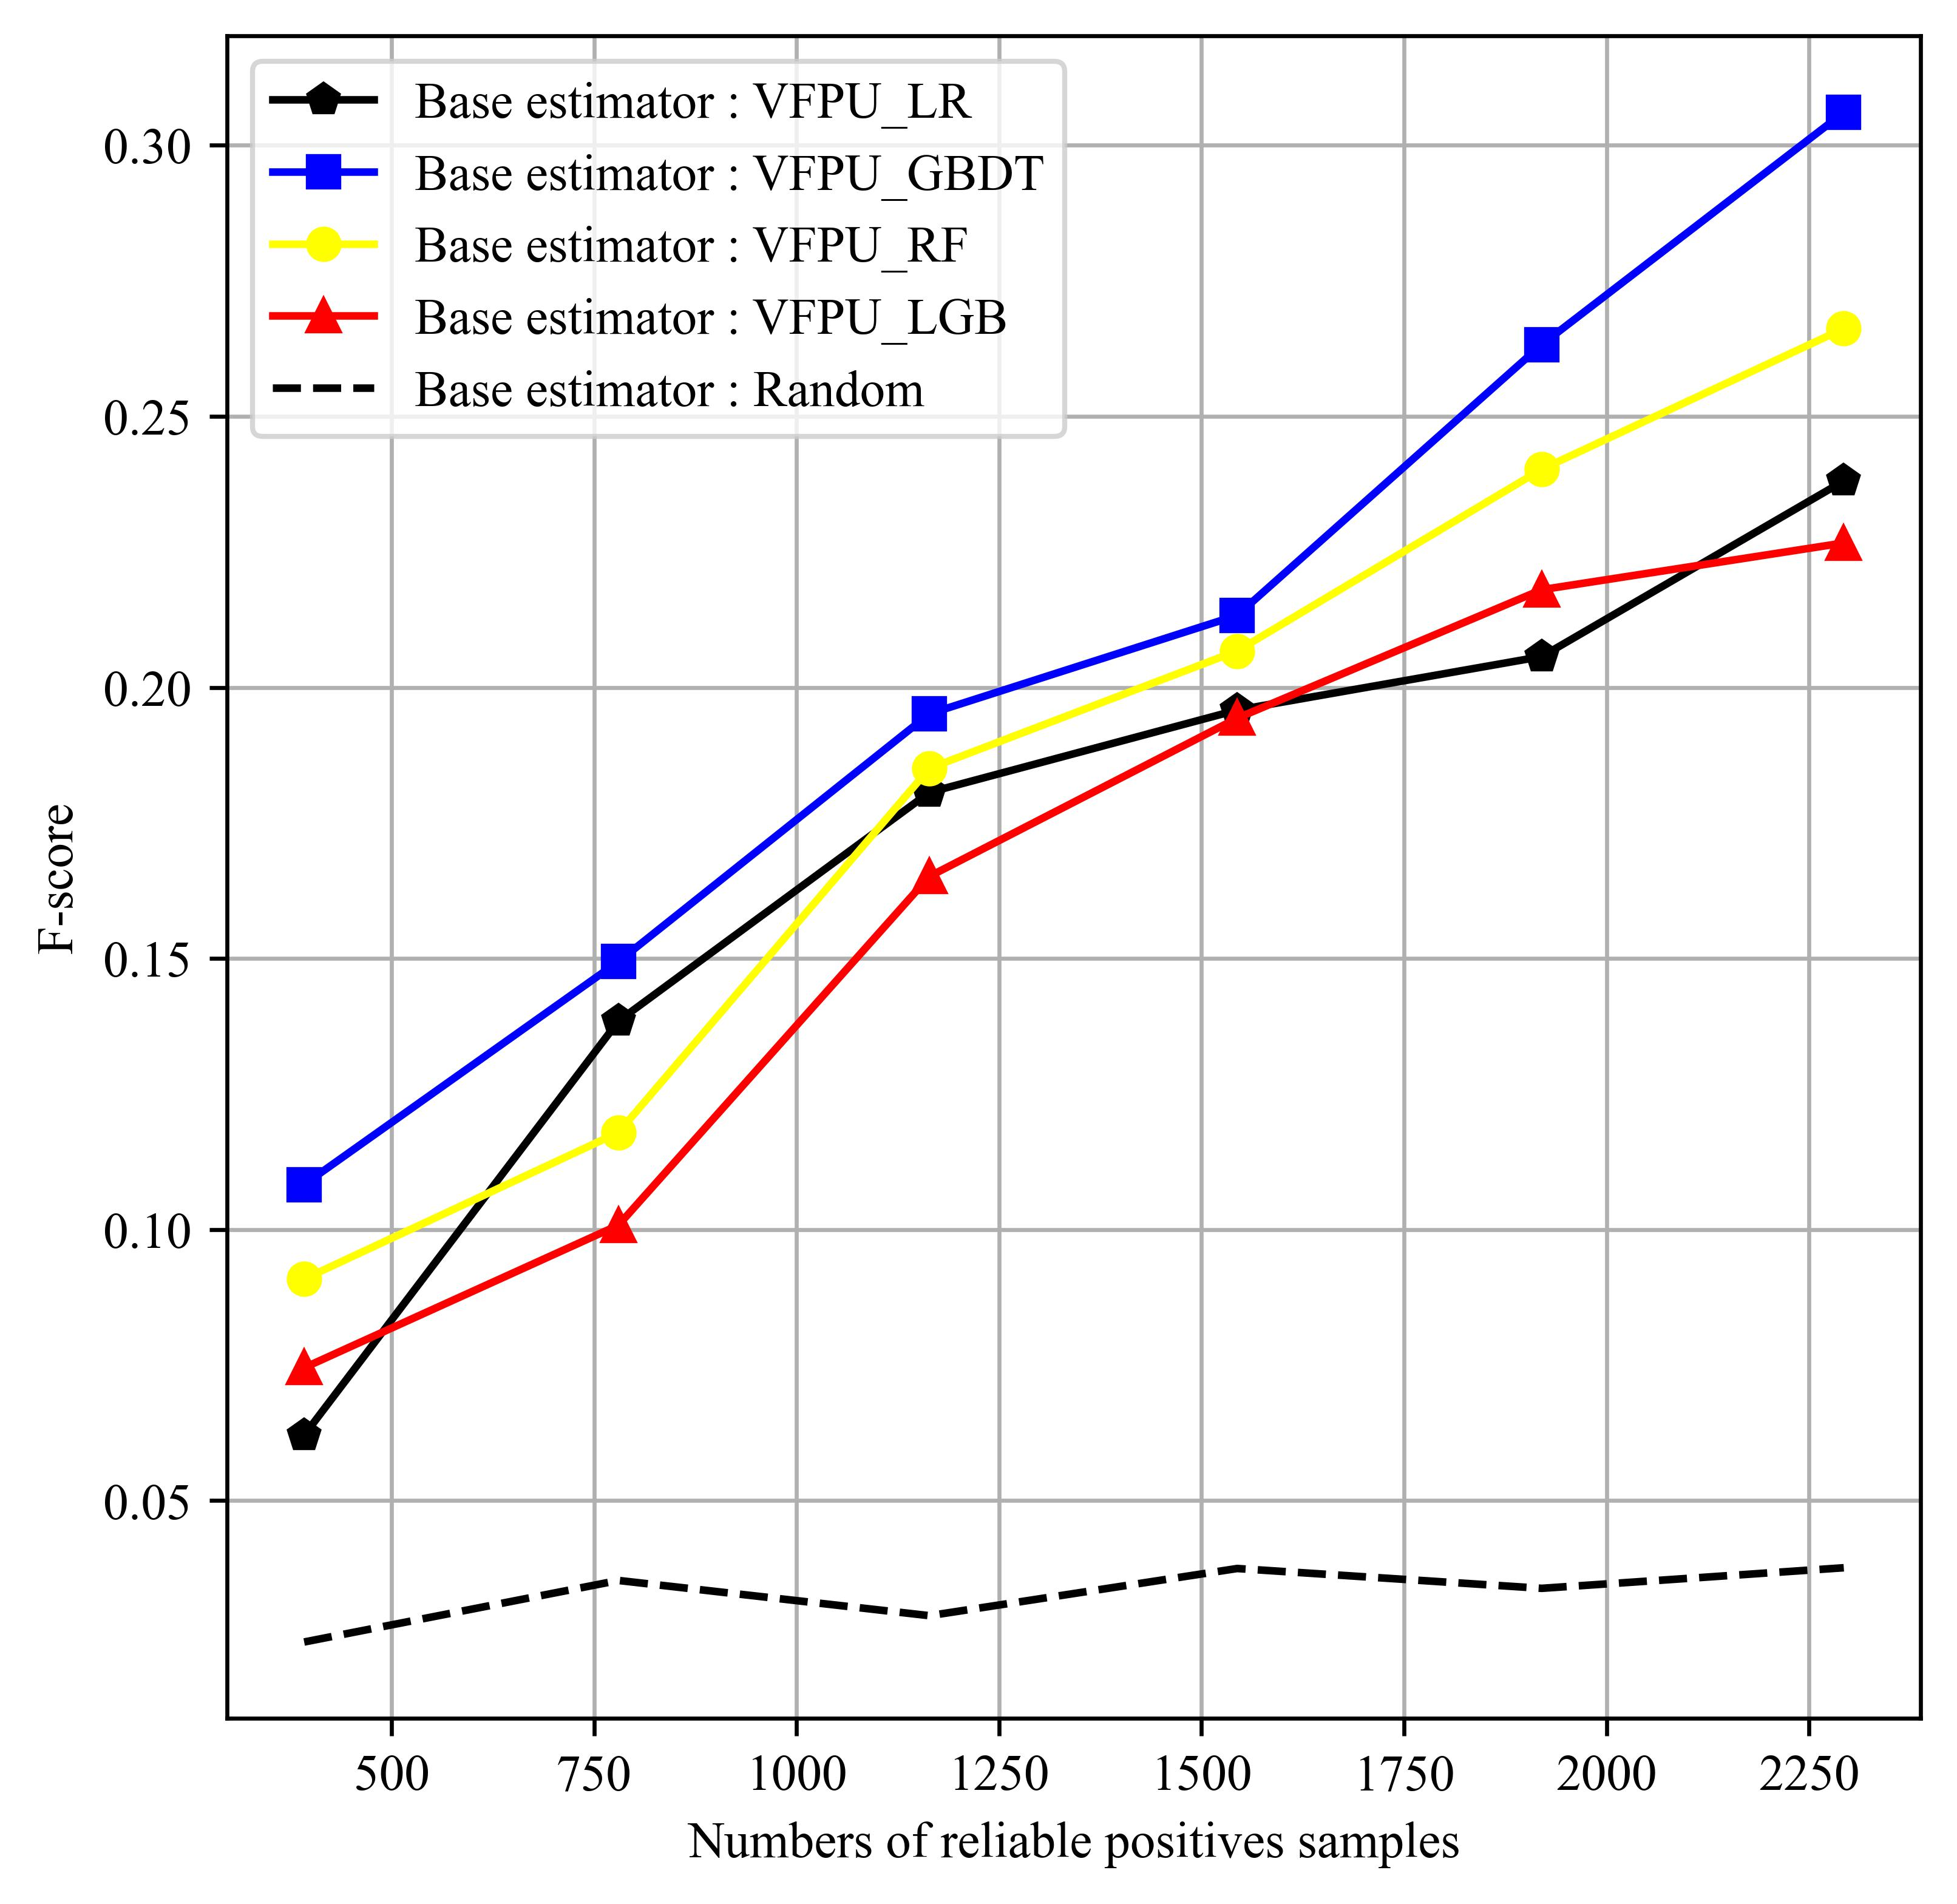
\includegraphics[width=0.9\textwidth,height=5.1cm]{chapters/imgs/Figure 3 (3) in JEPG format}
		\caption{F-score}
		\label{RQ2.2.sub3}
	\end{subfigure}
%\hfill
	\begin{subfigure}{0.45\textwidth}
		\centering
		\captionsetup{skip=4pt}
		\captionsetup{size=scriptsize}
		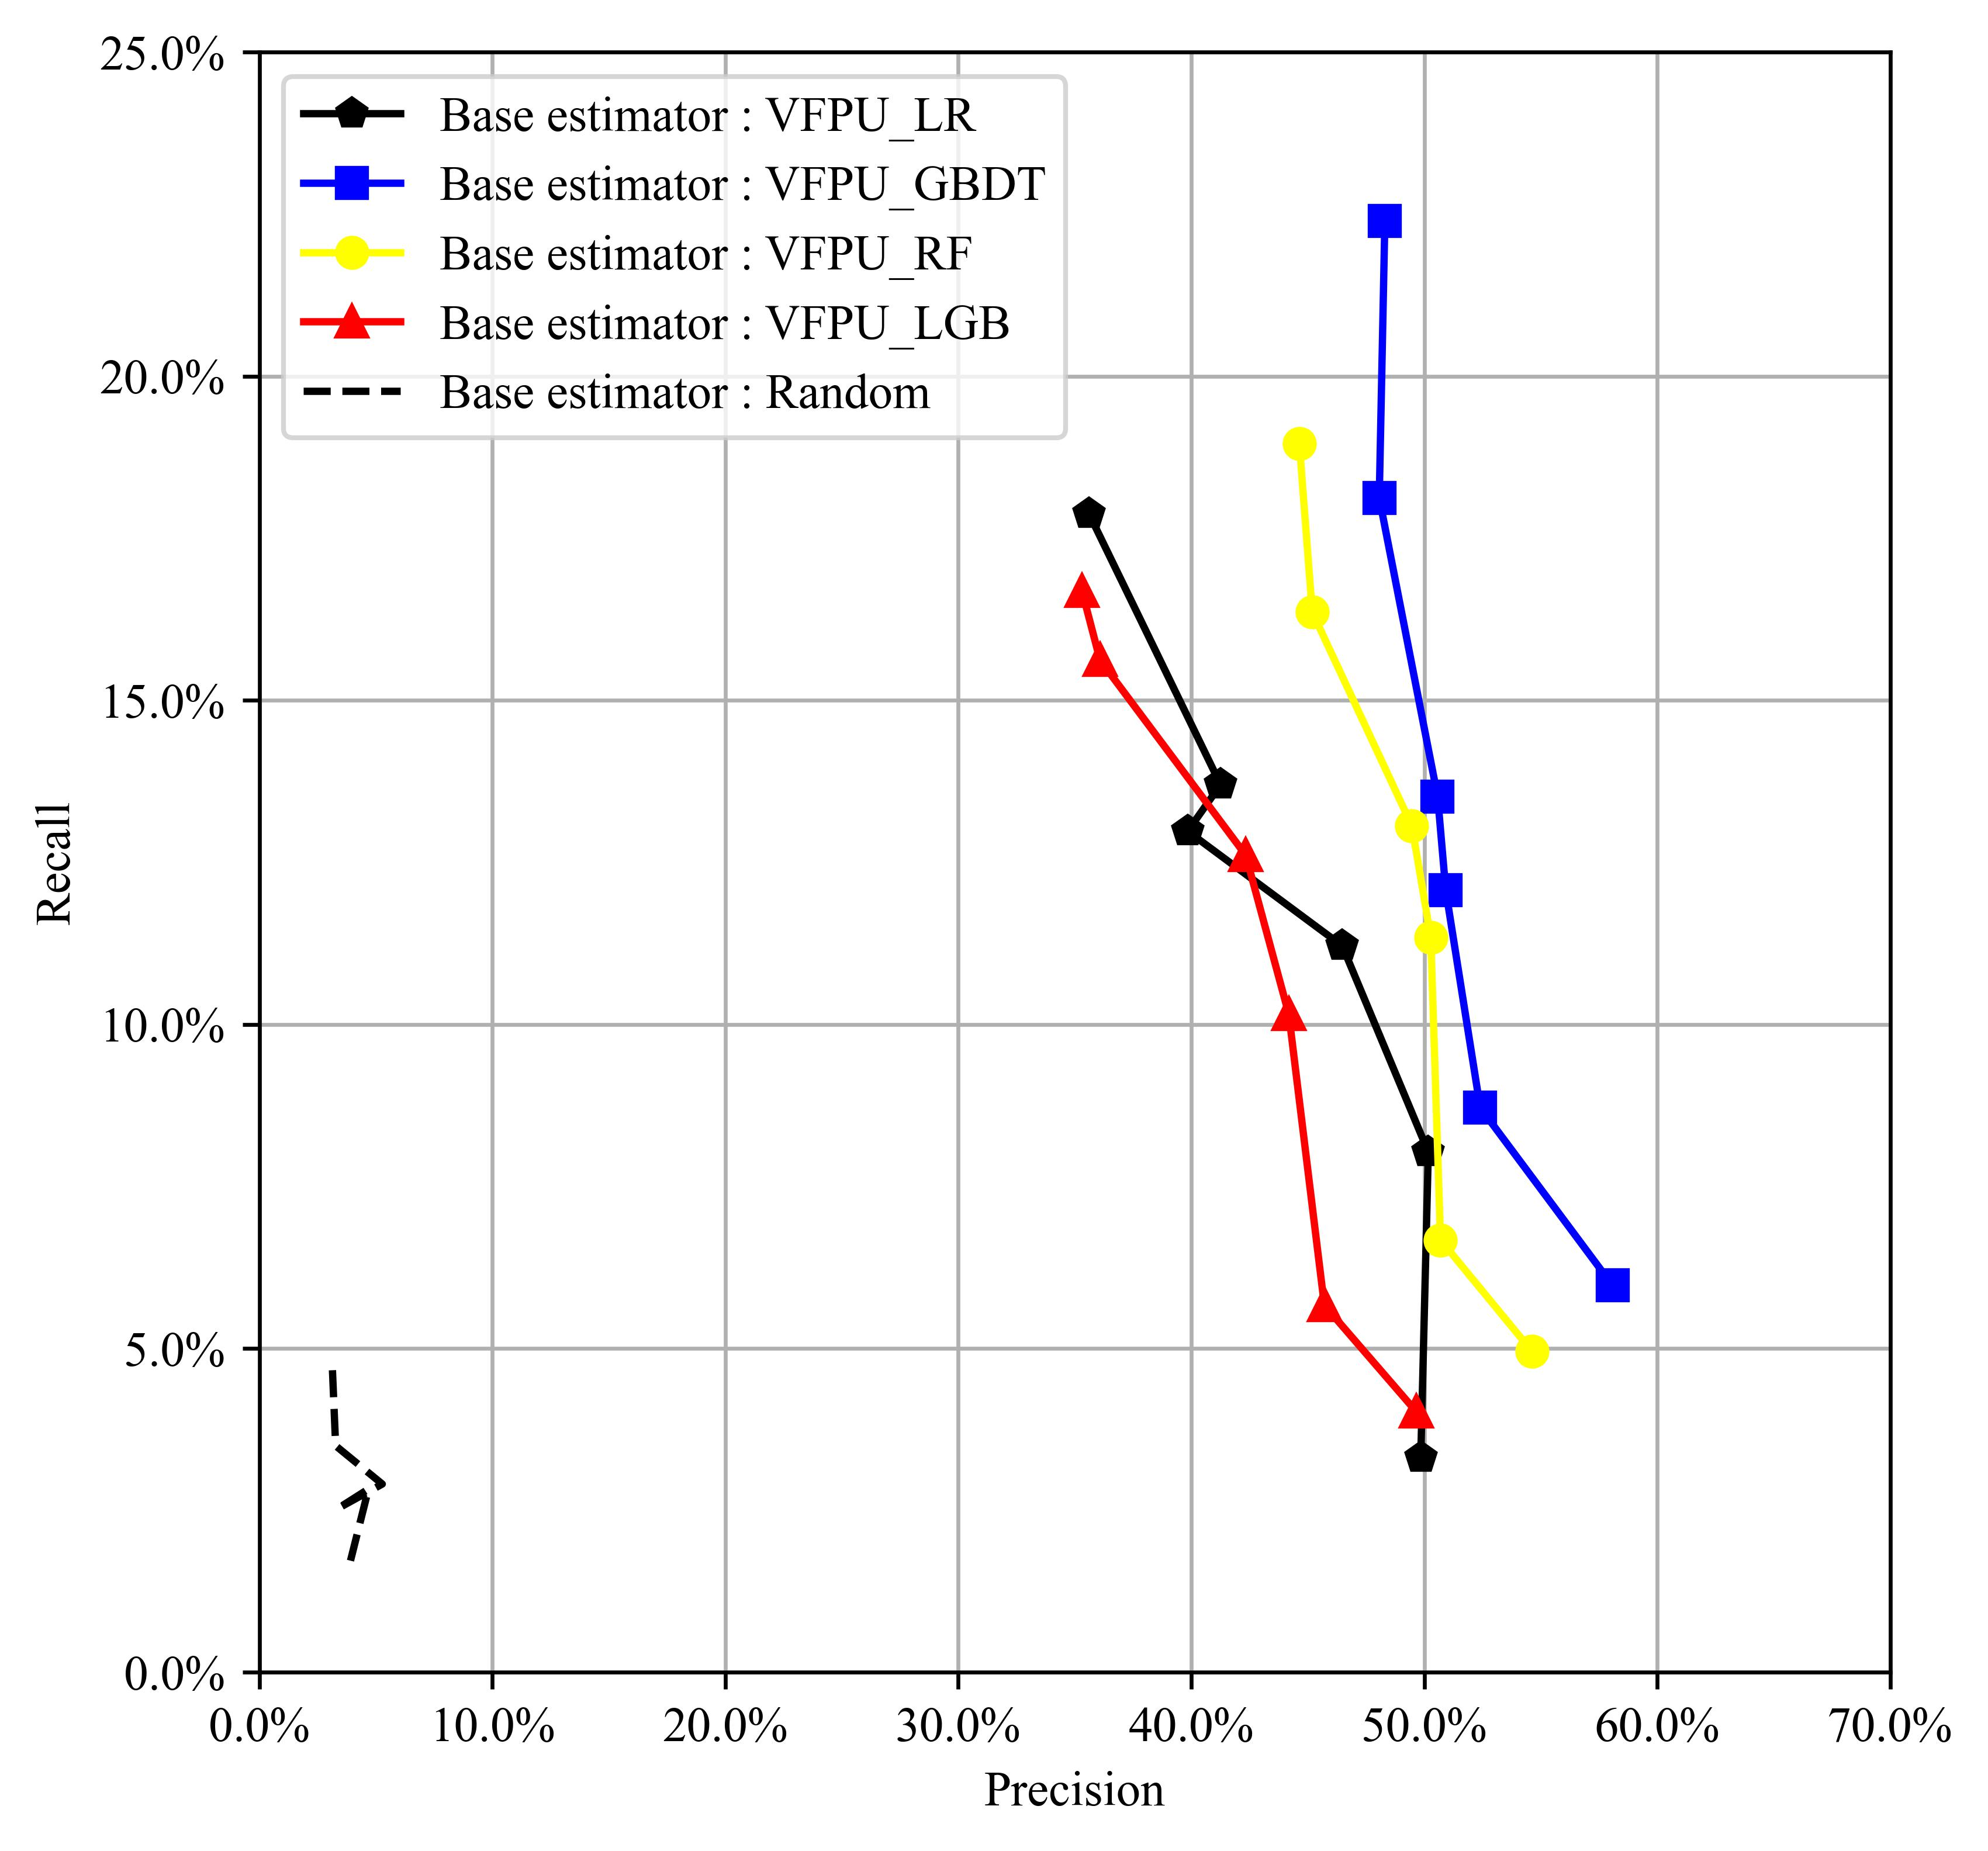
\includegraphics[width=0.9\textwidth,height=5.1cm]{chapters/imgs/Figure 3 (4) in JEPG format}
		\caption{Precision-Recall}
		\label{RQ2.2.sub4}
	\end{subfigure}
	
	\caption{Performance of Different Base Estimators with Varying Reliable Positive Samples: (1) Precision; (2) Recall; (3) F-score; (4) Precision-Recall (The Default of Credit Card Clients Dataset)}
	\bicaption[\xiaosi 不同基学器在不同可靠正样本数量下的性能]{\wuhao 不同基学器在不同可靠正样本数量下的性能:(1)精度;(2)召回率;(3)F-score;(4)精度-召回率(Credit 数据集)}{\wuhao Performance of Different Base Estimators with Varying Reliable Positive Samples: (1) Precision; (2) Recall; (3) F-score; (4) Precision-Recall (The Default of Credit Card Clients Dataset)}
    \label{RQ2.2}
\end{figure}

\begin{figure}[!htbp]
	\centering
	\captionsetup{size=footnotesize}
	\begin{subfigure}{0.45\textwidth}
		\centering
		\captionsetup{skip=2pt}
		\captionsetup{size=scriptsize}
		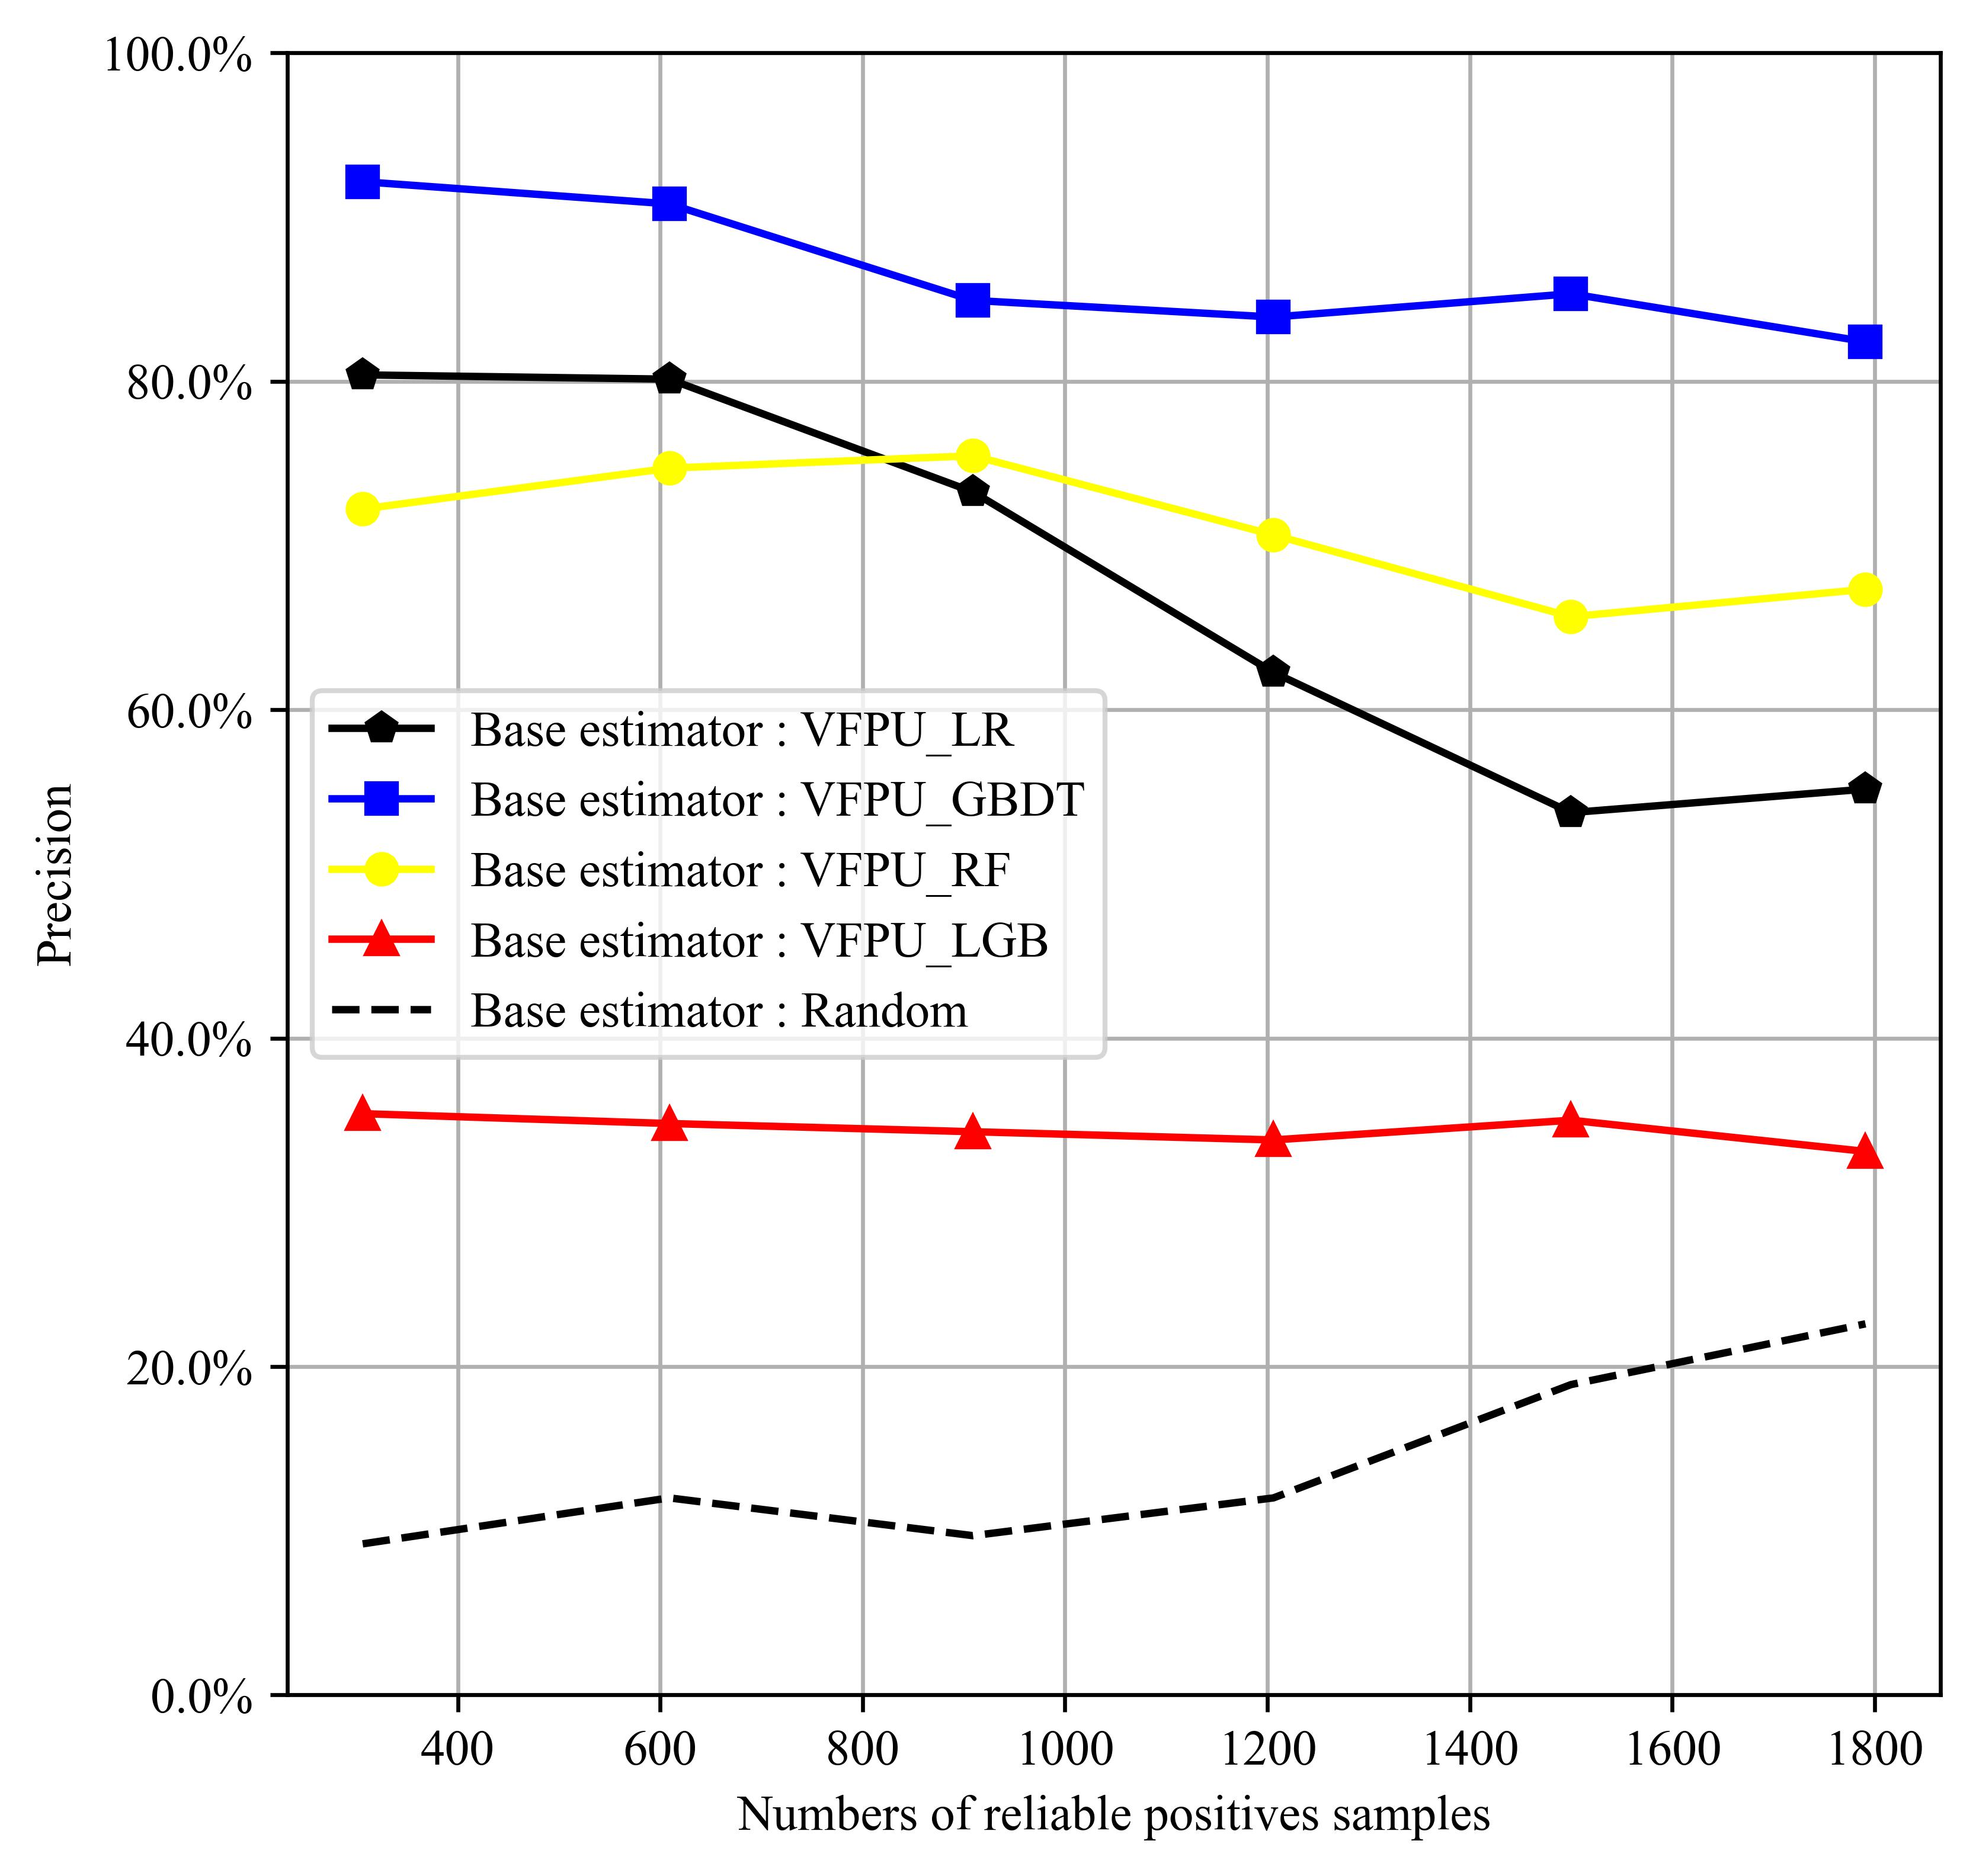
\includegraphics[width=0.9\textwidth,height=5.1cm]{chapters/imgs/Figure 4 (1) in JEPG format}
		\caption{Precision}
		\label{RQ2.3.sub1}
	\end{subfigure}
%\hfill
	\begin{subfigure}{0.45\textwidth}
		\centering
		\captionsetup{skip=2pt}
		\captionsetup{size=scriptsize}
		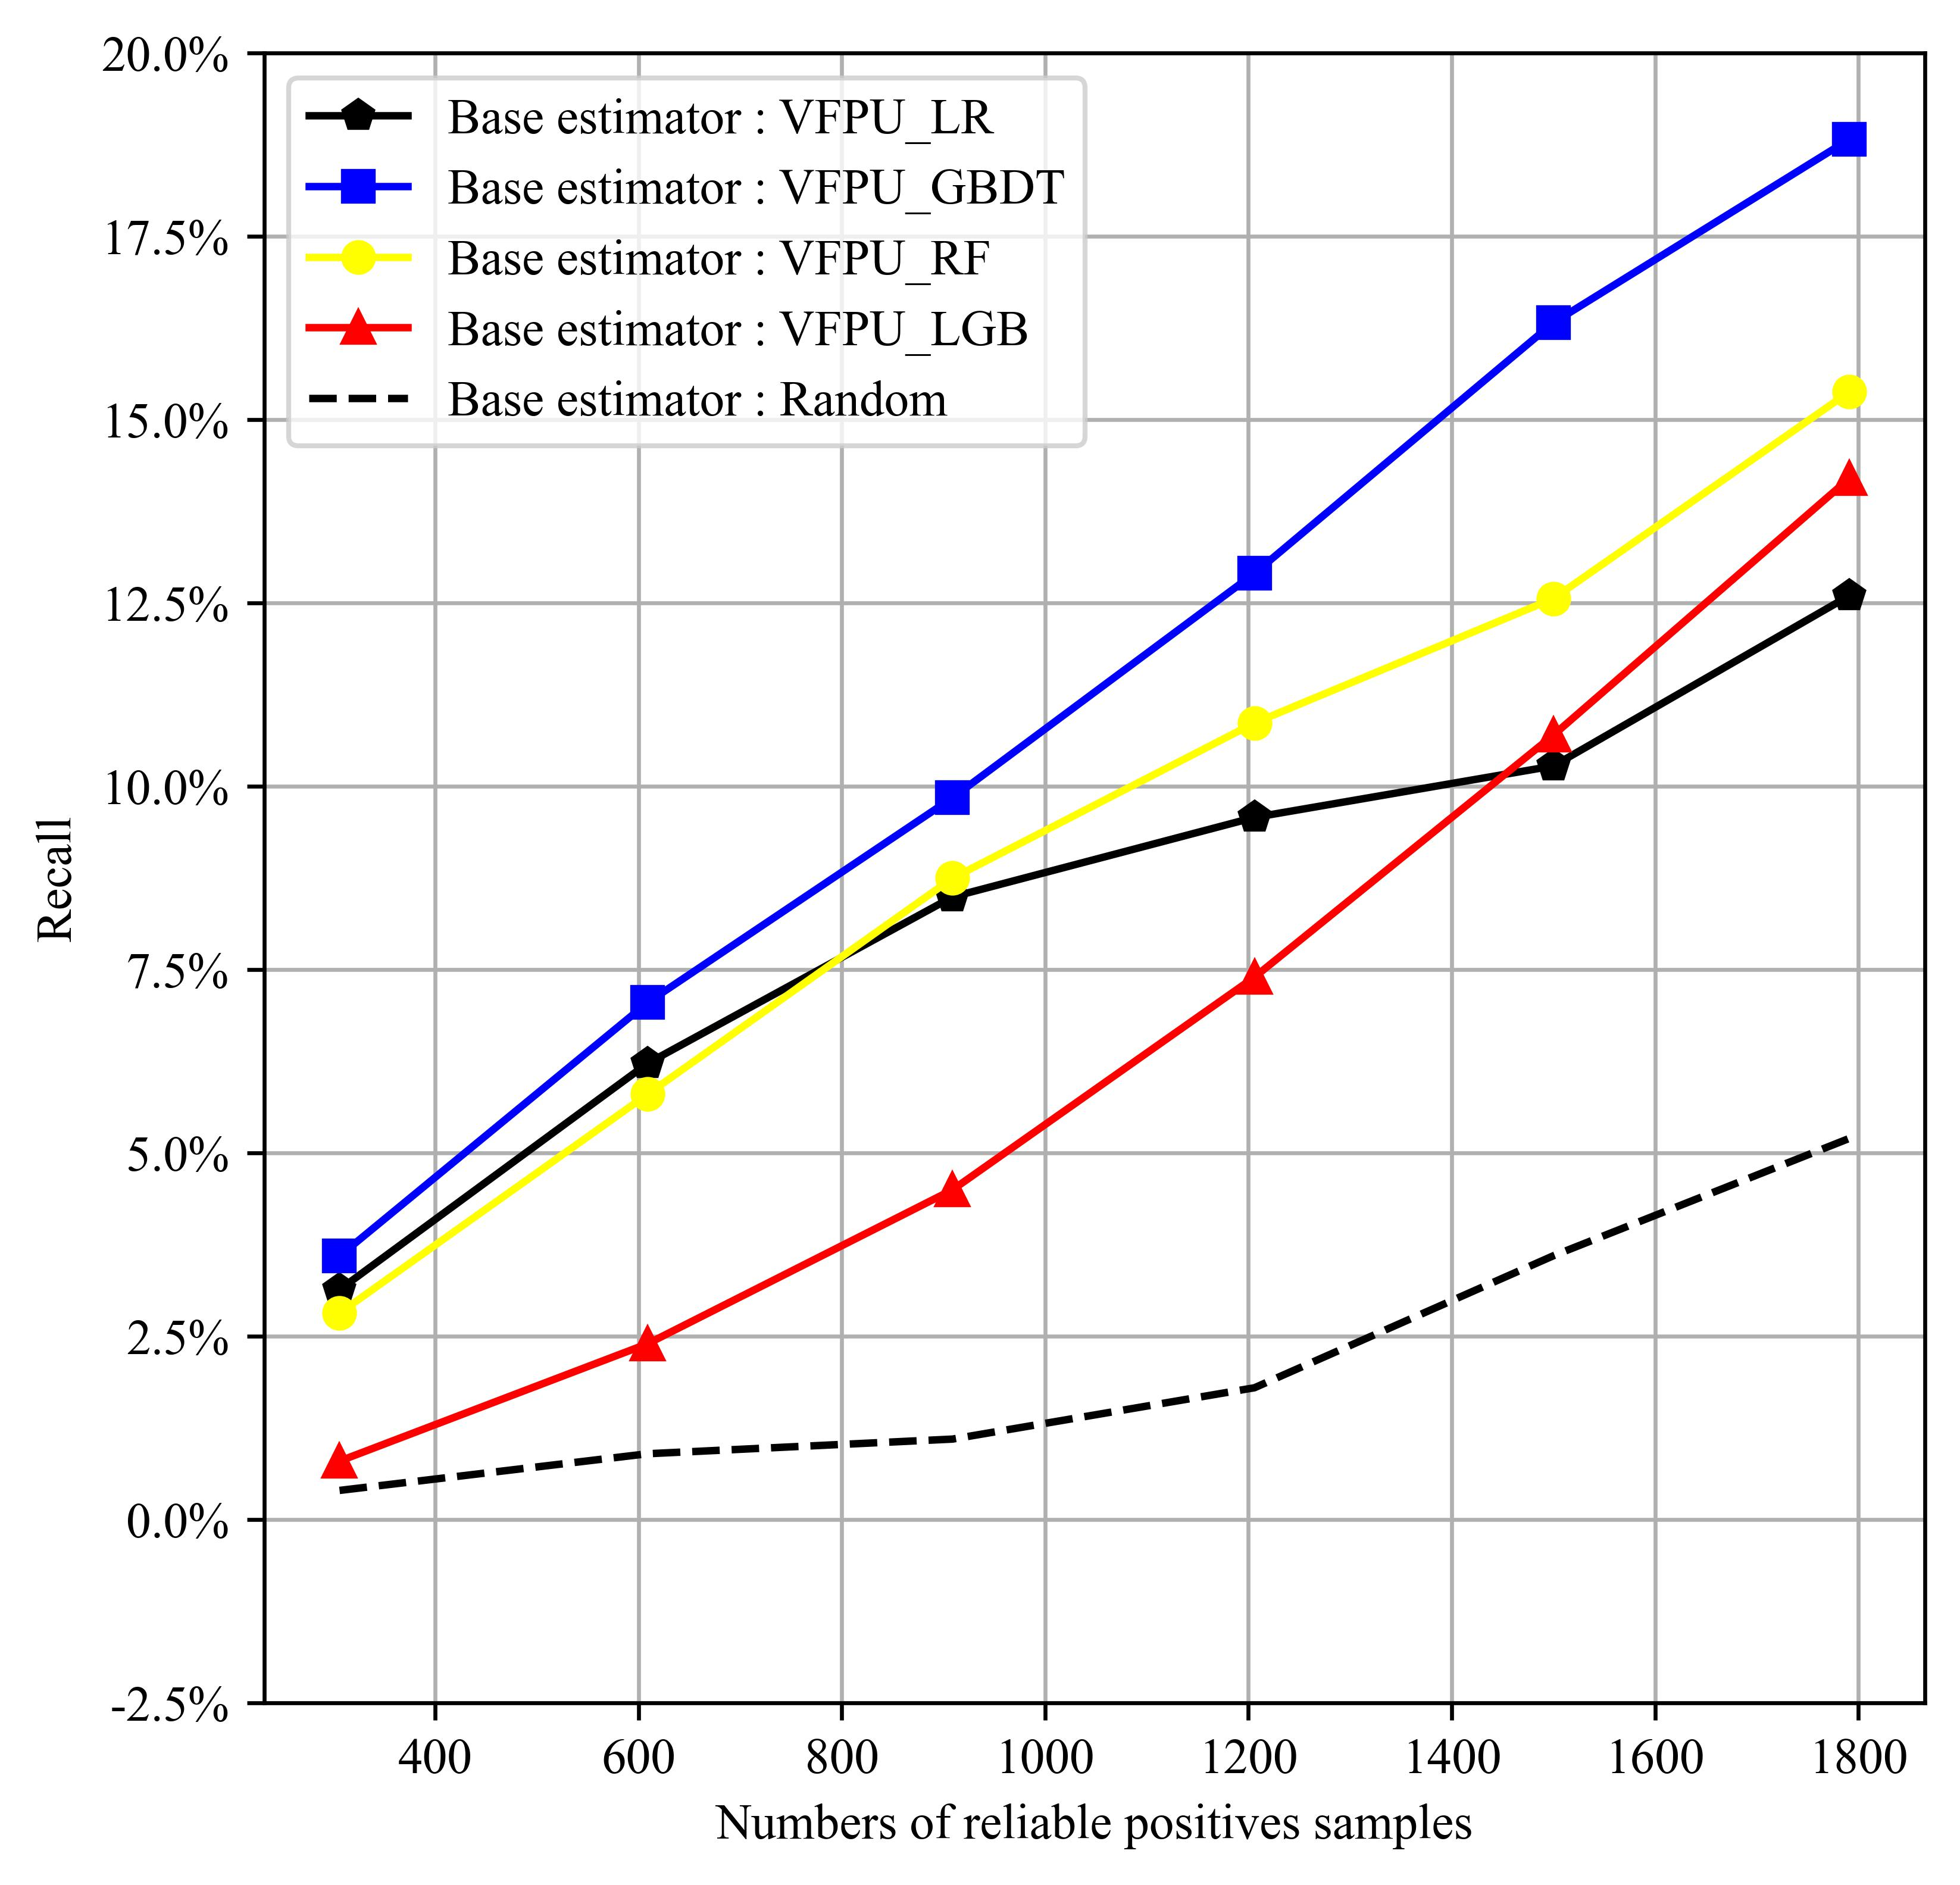
\includegraphics[width=0.9\textwidth,height=5.1cm]{chapters/imgs/Figure 4 (2) in JEPG format}
		\caption{Recall}
		\label{RQ2.3.sub2}
	\end{subfigure}
	
%	\vspace{0.05cm}
	
	\begin{subfigure}{0.45\textwidth}
		\centering
		\captionsetup{skip=2pt}
		\captionsetup{size=scriptsize}
		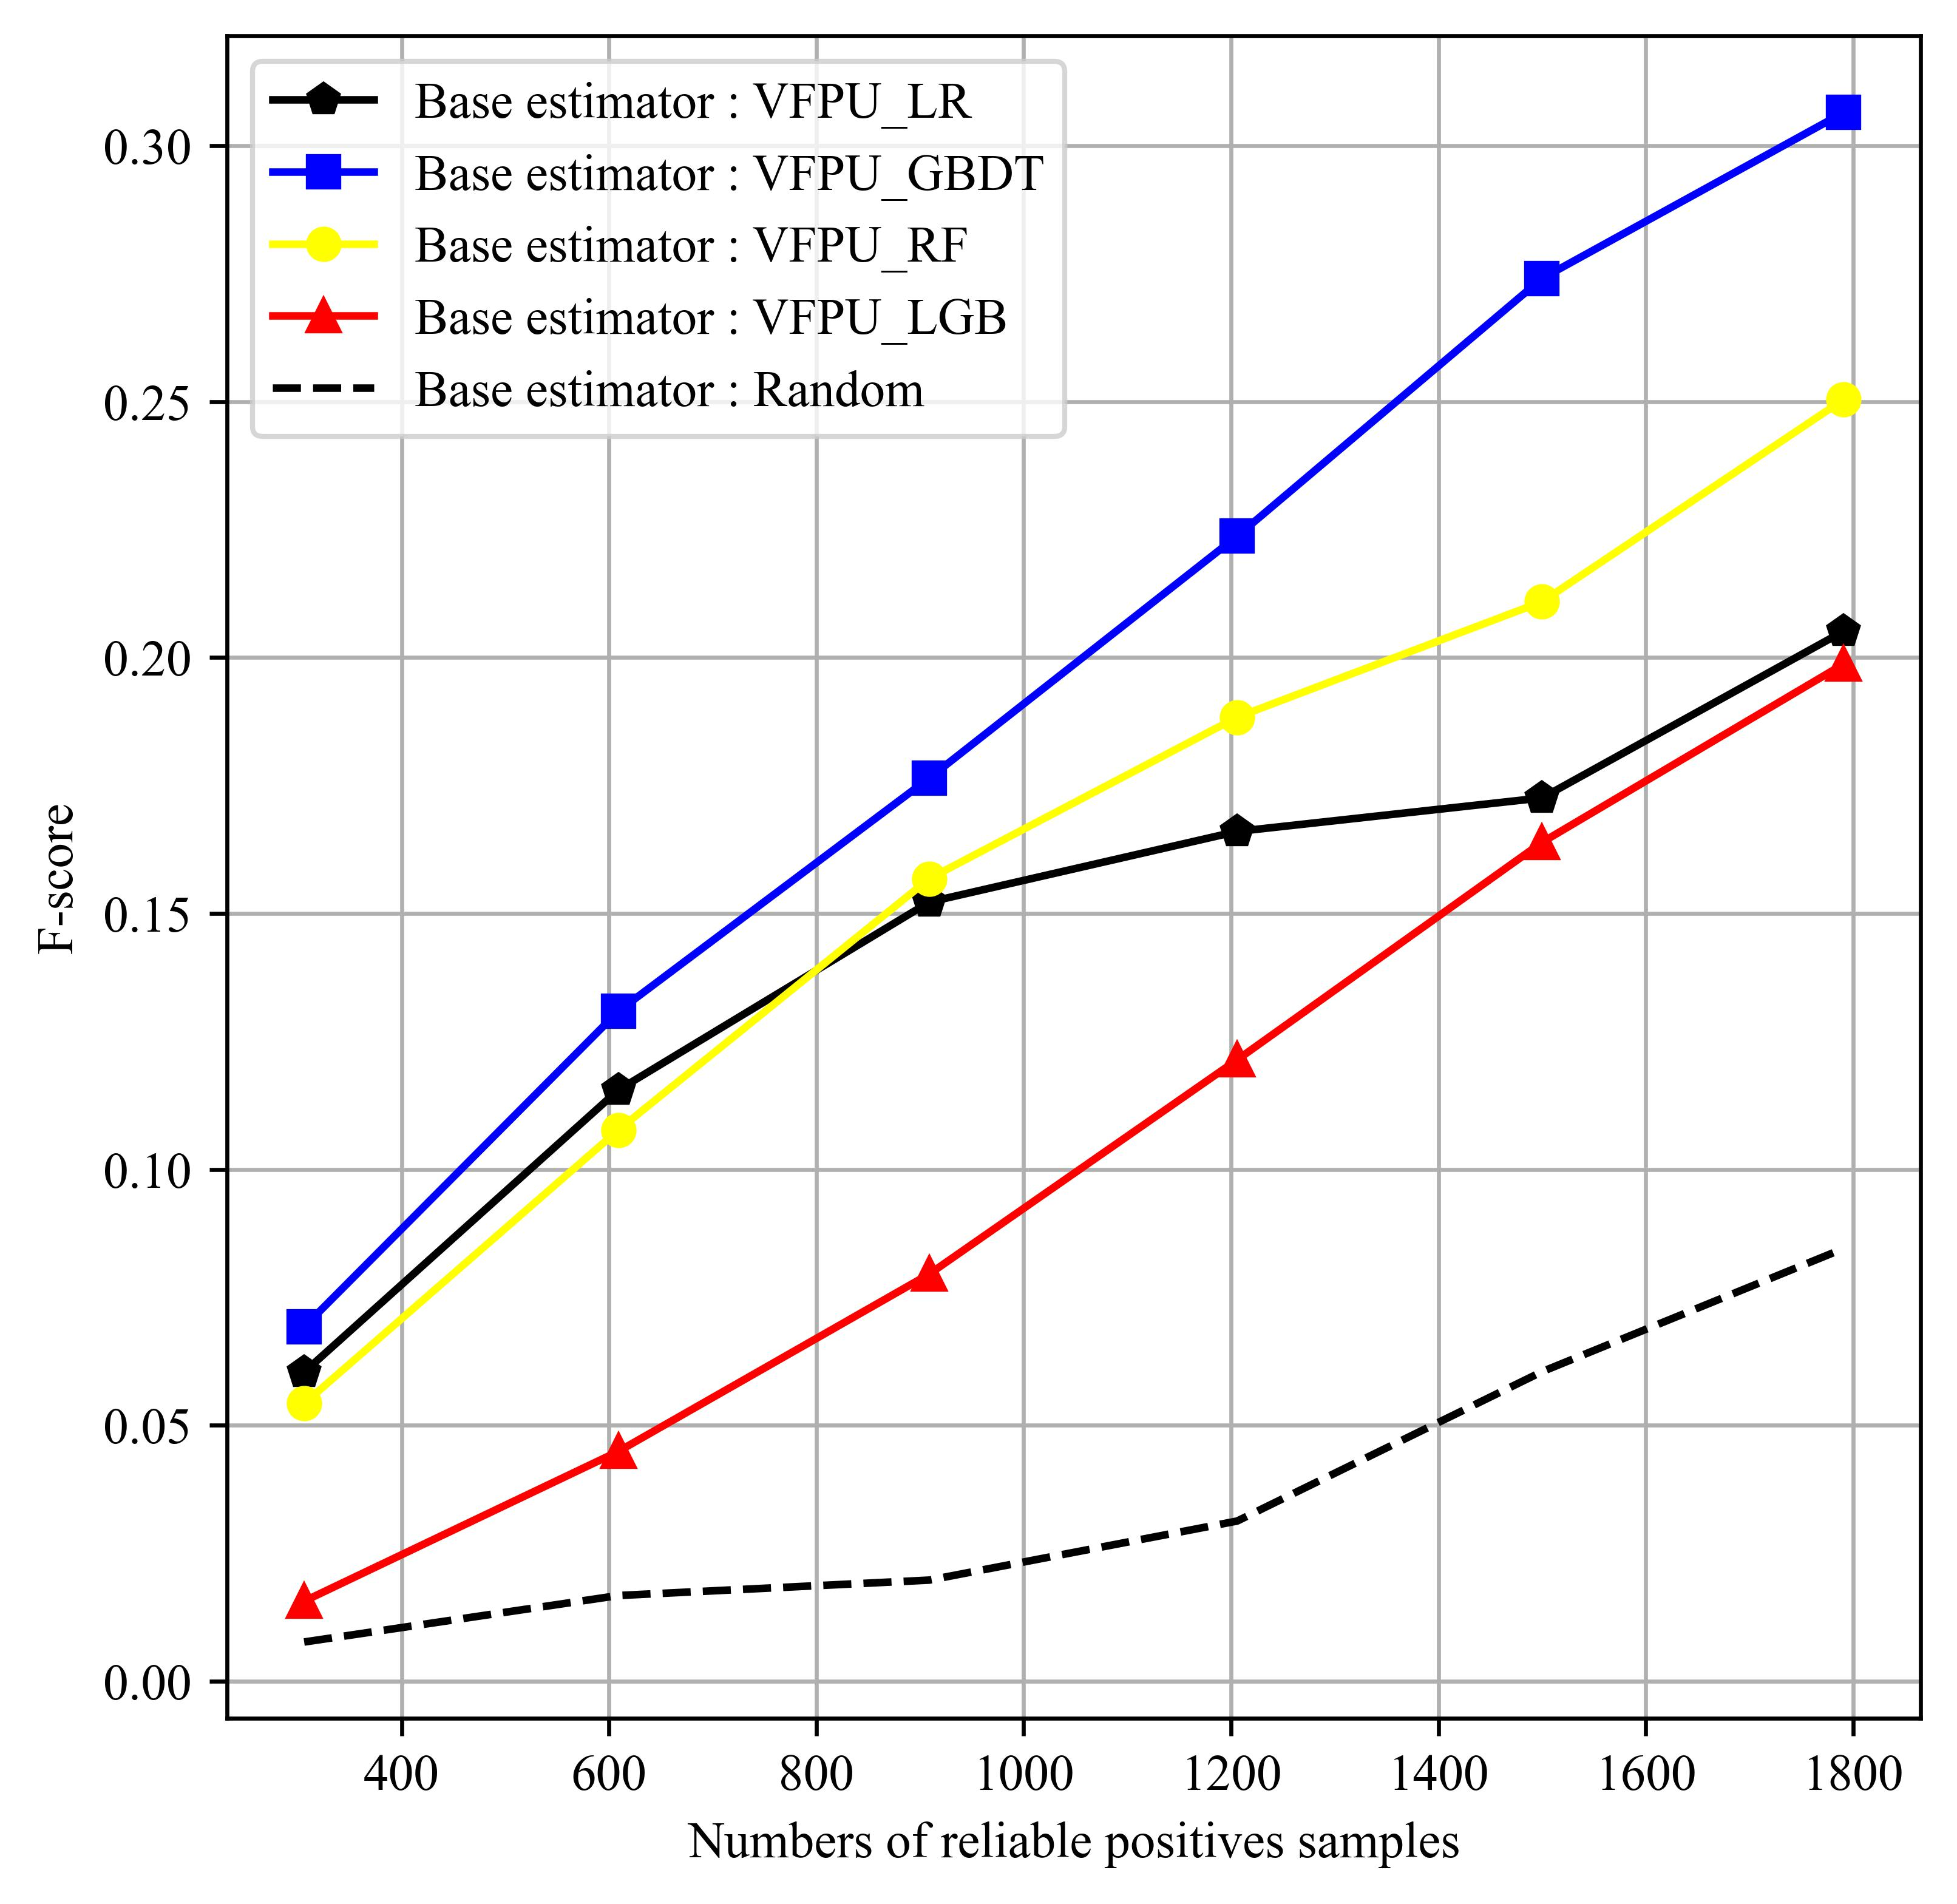
\includegraphics[width=0.9\textwidth,height=5.1cm]{chapters/imgs/Figure 4 (3) in JEPG format}
		\caption{F-score}
		\label{RQ2.3.sub3}
	\end{subfigure}
%\hfill
	\begin{subfigure}{0.45\textwidth}
		\centering
		\captionsetup{skip=2pt}
		\captionsetup{size=scriptsize}
		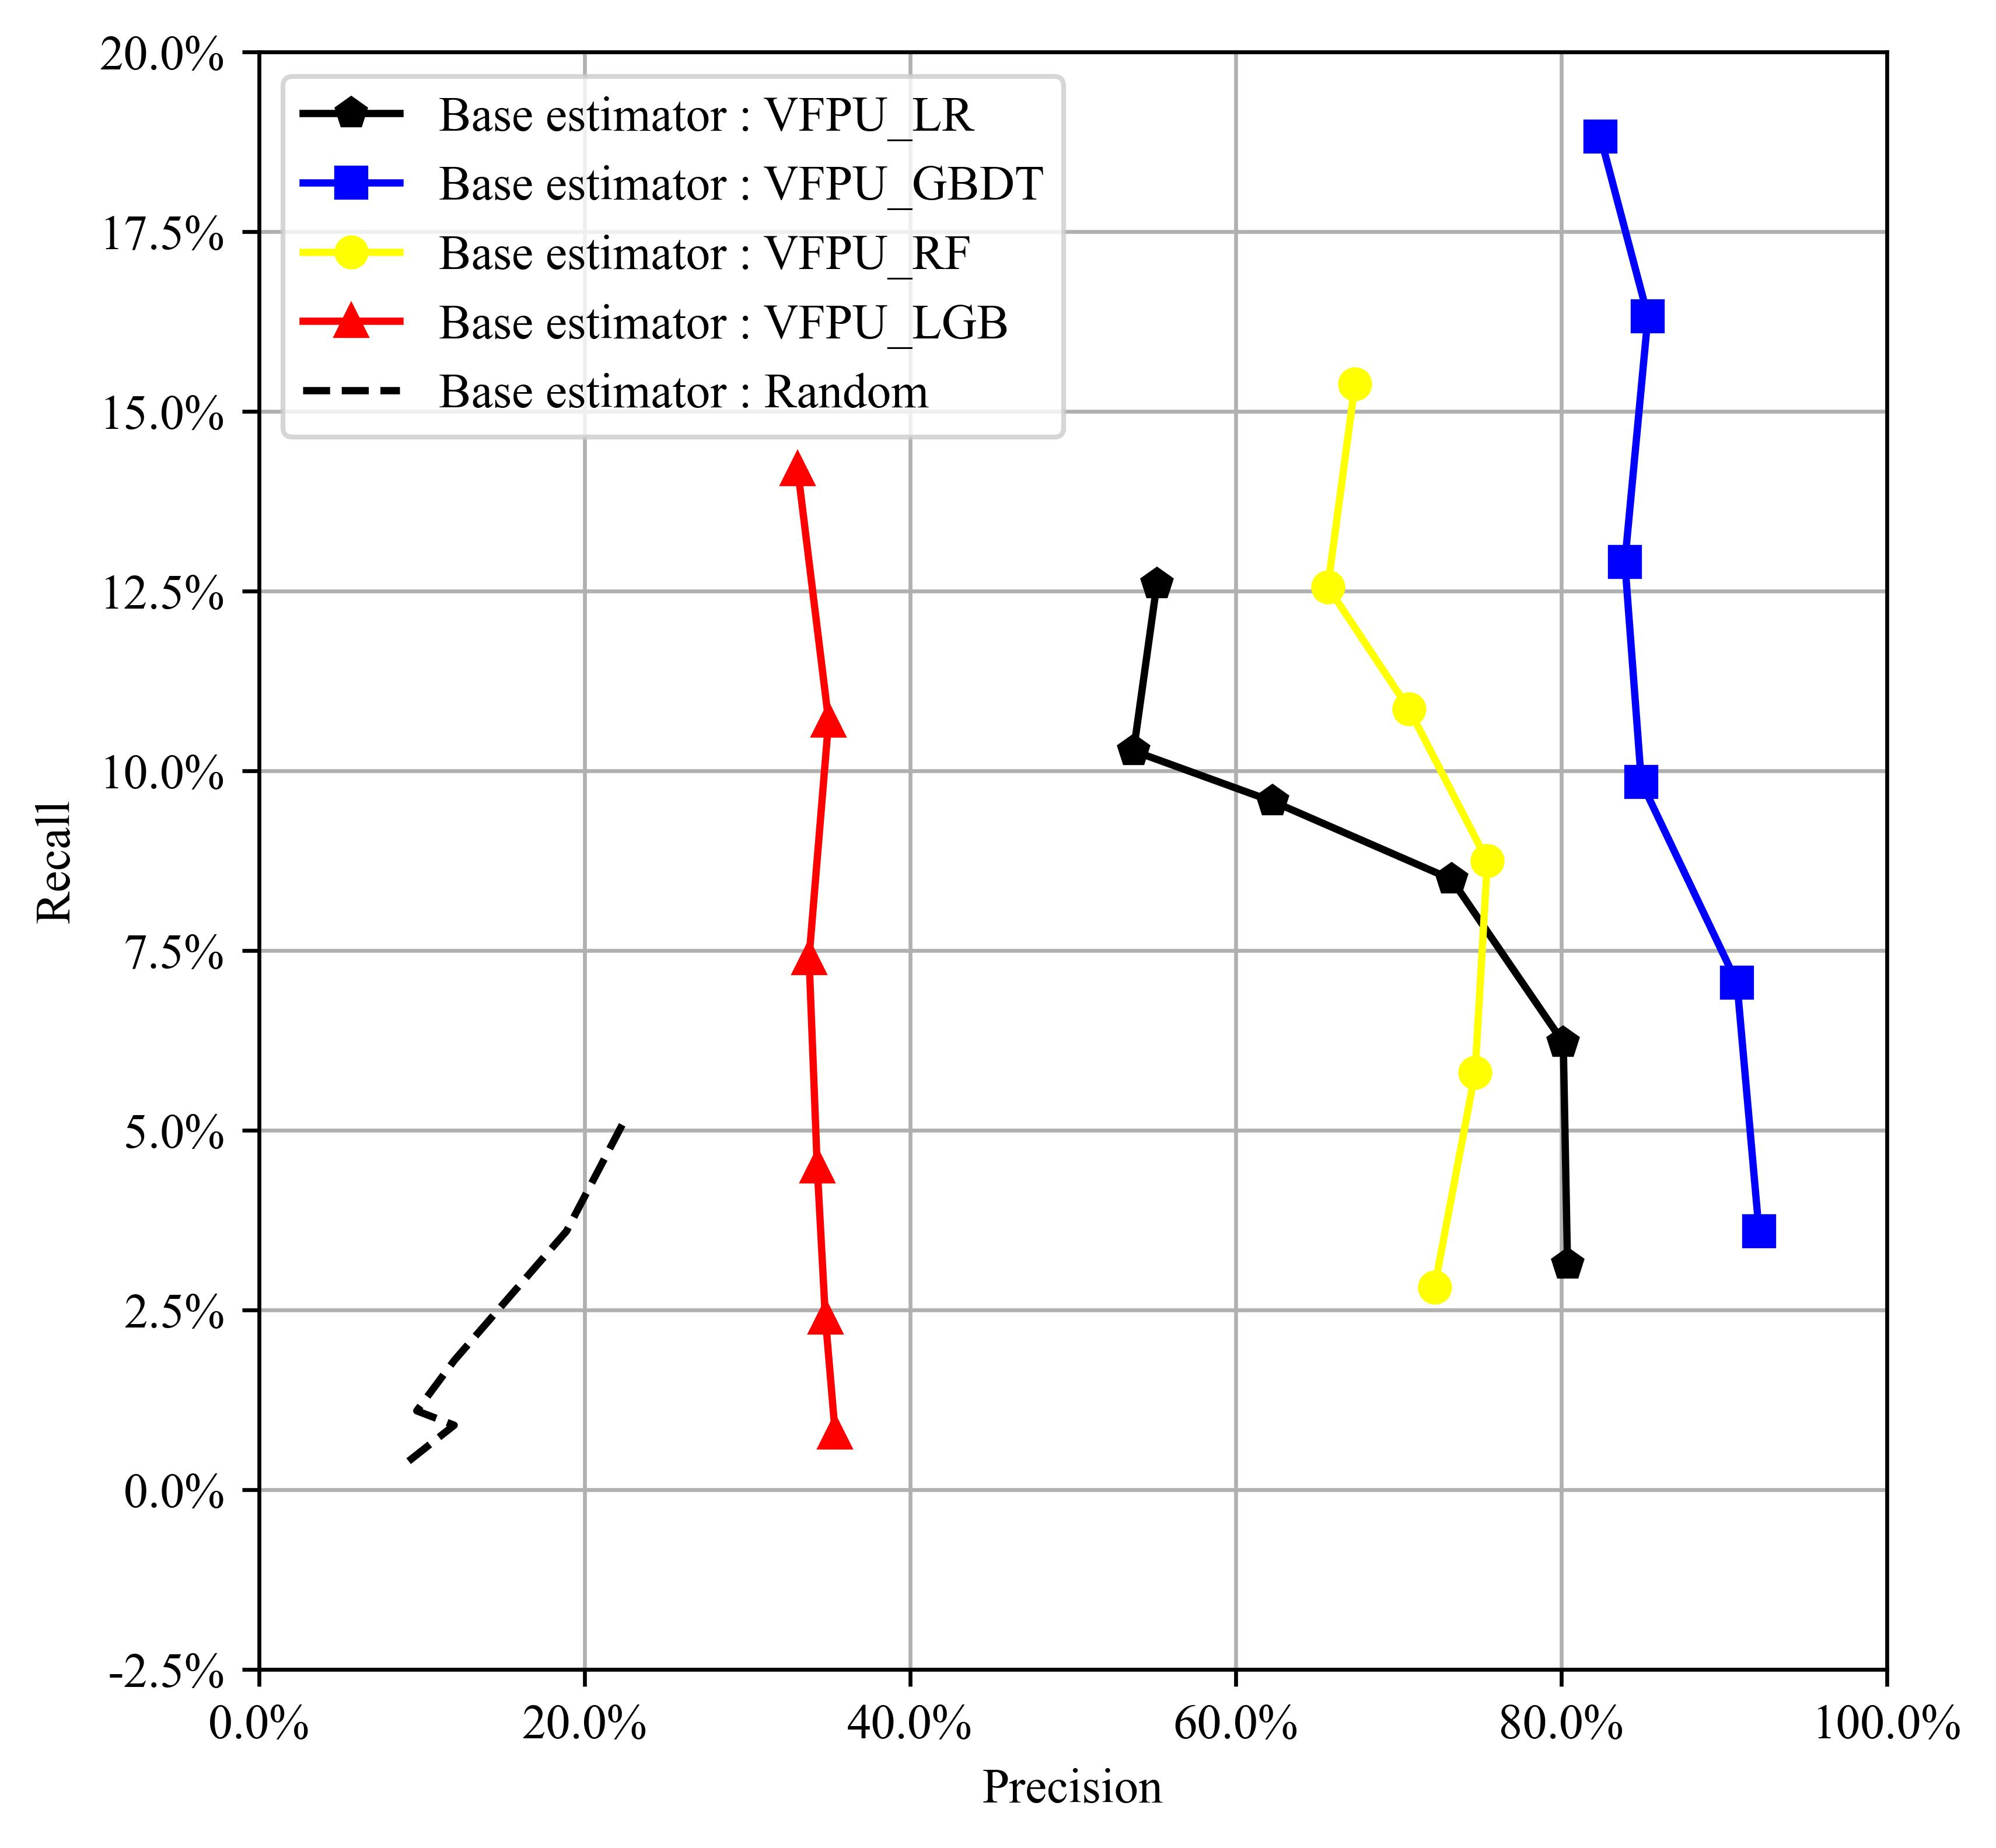
\includegraphics[width=0.9\textwidth,height=5.1cm]{chapters/imgs/Figure 4 (4) in JEPG format}
		\caption{Precision-Recall}
		\label{RQ2.3.sub4}
	\end{subfigure}
	\bicaption[\xiaosi 不同基学器在不同可靠正样本数量下的性能]{\wuhao 不同基学器在不同可靠正样本数量下的性能:(1)精度;(2)召回率;(3)F-score;(4)精度-召回率(Census 数据集)}{\wuhao Performance of Different Base Estimators with Varying Reliable Positive Samples: (1) Precision; (2) Recall; (3) F-score; (4) Precision-Recall (The Adult Census Dataset)}
    \label{RQ2.3}
\end{figure}

\begin{figure}[!htbp]
	\centering
	\captionsetup{size=footnotesize}
	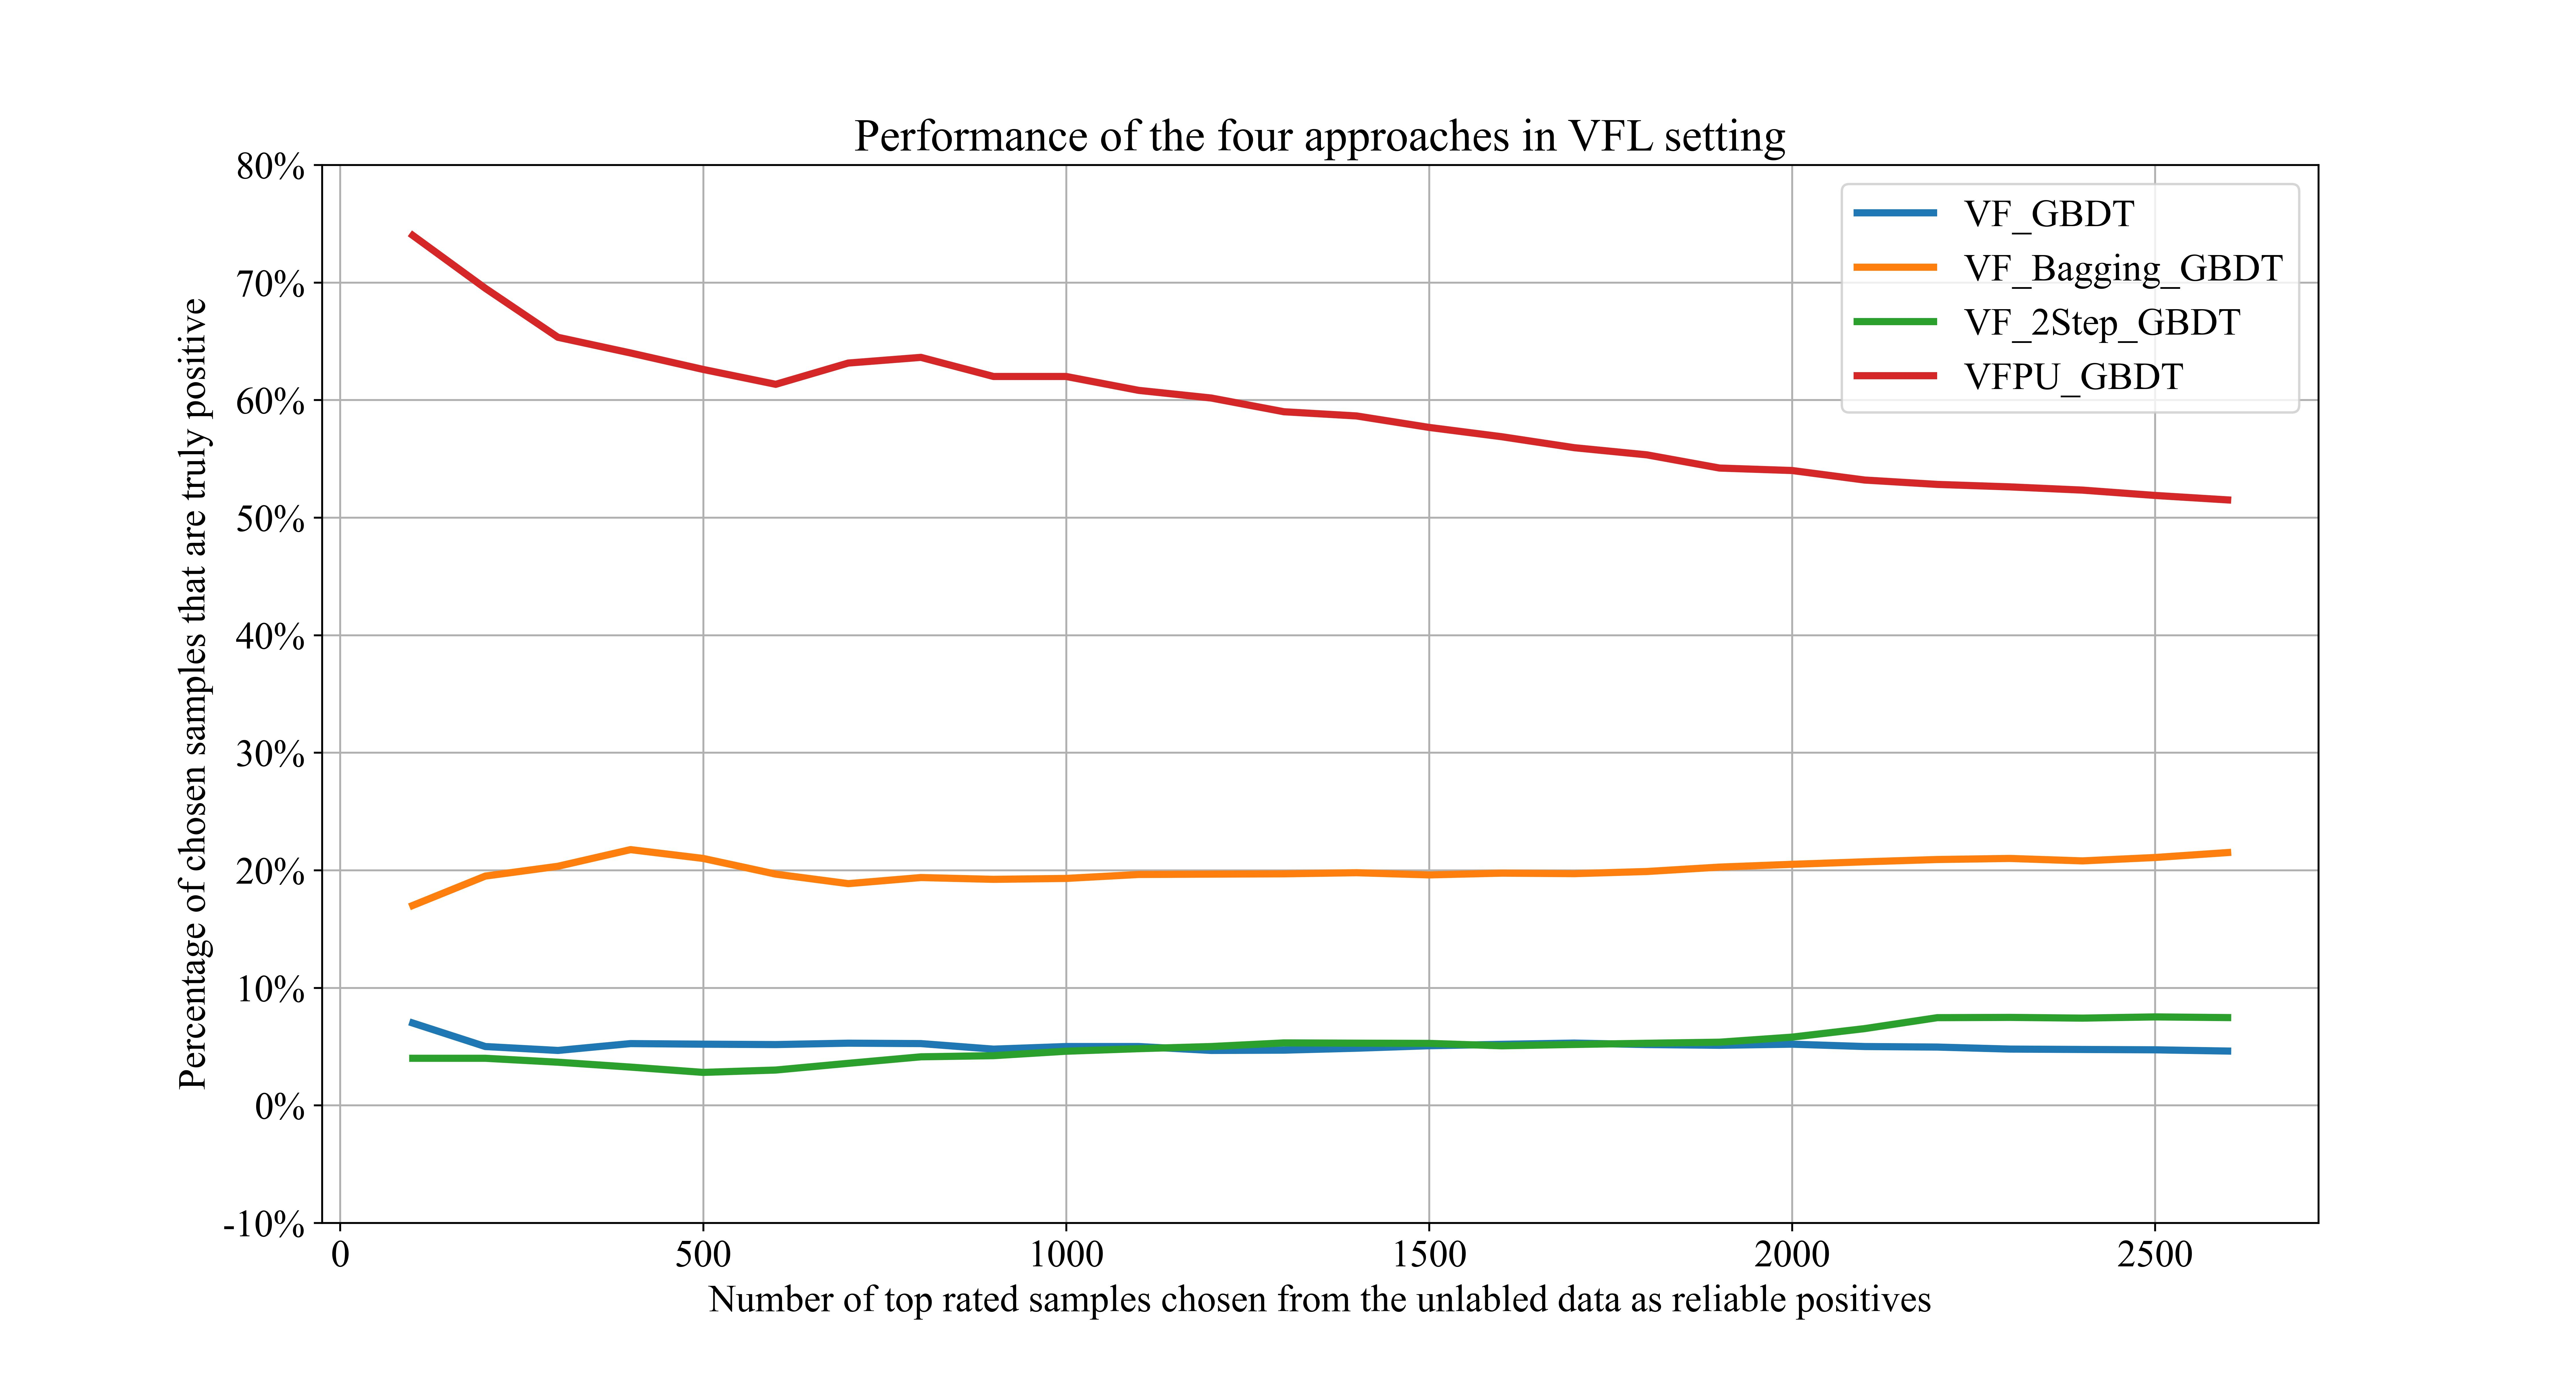
\includegraphics[width=0.9\textwidth,height=9cm]{chapters/imgs/Figure 5 in JPEG format}
    \bicaption[\xiaosi 在纵向联邦学习中通过不同的半监督方法获得的准确推荐百分比]{\wuhao 在纵向联邦学习中通过不同的半监督方法获得的准确推荐百分比(Bank数据集)}{\wuhao The accurate recommendations percentage by Different Semi-supervised Methods in VFL (The Bank Marketing Dataset)}
	\label{fig:GBDT}
\end{figure}